\section{Audio-Based Navigation}\label{sec:AudioBasedNavigation}
Audio-based navigation, as with any robot system, can be subdivided in several smaller systems, components or problems. One general and widely spread approach to this system decomposition is SPA, or sense-plan-act \cite{AudioBasedNavigation:SensePlanAct}. However, it is commonly -- in navigation contexts -- further divided further into SPPA, or sense-perceive-plan-act, as seen in Figure \ref{fig:AutonomousNavigationOverview} \cite{AudioBasedNavigation:AutonomousNavigation}.

\begin{figure}[H]
    \centering
    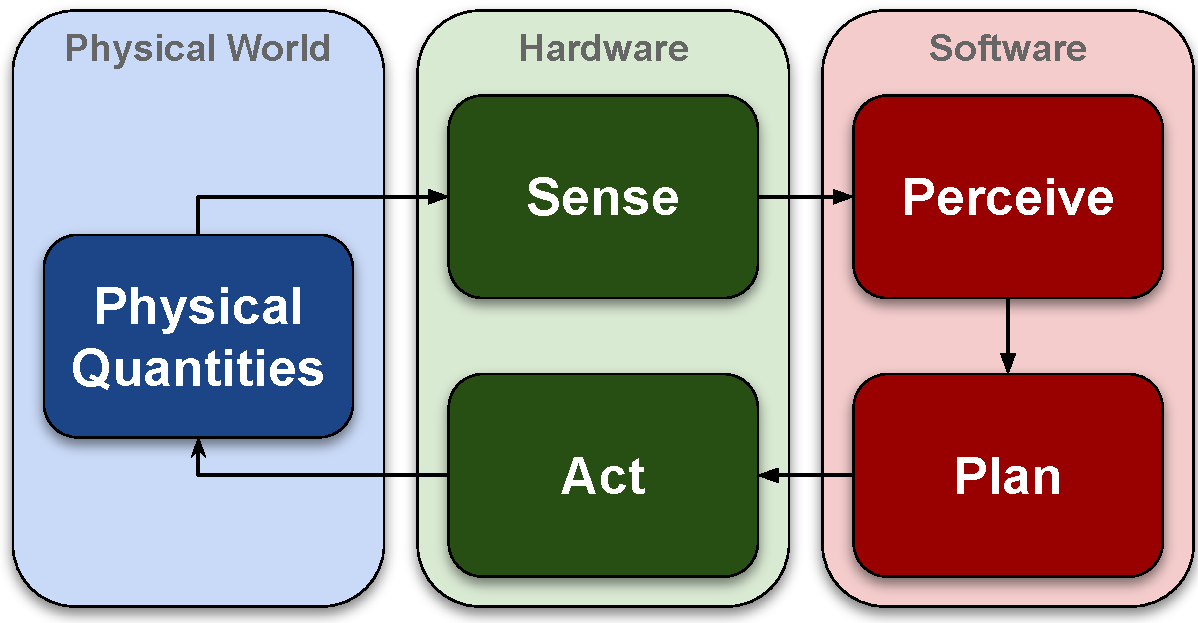
\includegraphics[width=.8\textwidth]{figures/1Problem_analysis/Autonomous Navigation - Overview.pdf}
    \caption{The SPPA system decomposition}
    \label{fig:AutonomousNavigationOverview}
\end{figure}

This section aims to describe the topics in Figure \ref{fig:AutonomousNavigationOverview} in further detail and will outline the material, starting from "Physical Quantities", in the following subsections.

\subsection{Sound and Its Behaviour}\label{subsec:Sound}
Acoustics, being the field that deals with the multiple aspects related to sound, is applied in many architectural, military, musical, medical, and more recently robotic contexts. The understanding of sound have developed to the point where it can be utilised in new ways within the engineering field. To utilise sound in this context it is necessary to understand how sound is created, transmitted, received and how it acts in various situations. This section will cover the basics of sound, while also analysing the most relevant topics related to sound in a robotic application. \cite{Acoustics:Handbook_of_Acoustics}

\subsubsection{Defining Properties}
% What is sound
By scientific definition, sound is a disturbance that travels through a given medium and is categorised as a mechanical wave. In other words, it is the transportation of energy by the vibration or displacement of particles in the medium in which sound is propagating. Typically, the sound waves from a source will be radiating in all directions and the amplitude will depend on the direction and distance from the source. When dealing with the propagation of sound in fluids such as air, the vibration of particles (i.e. air molecules) causes a repeating sequence of high- and low pressures\footnote{These high- and low pressures are also known as compressions and rarefactions, respectively.}, referred to as pressure waves. As the movement of these particles occurs along the direction of energy transportation, sound waves can be further categorised as longitudinal waves. An illustration of sound propagation in air from a planar view can be seen in Figure \ref{Sound:sound_propagation}. \cite{Acoustics:Definition_of_sound1, Acoustics:Definition_of_sound2} 

\begin{figure}[H]
    \centering
    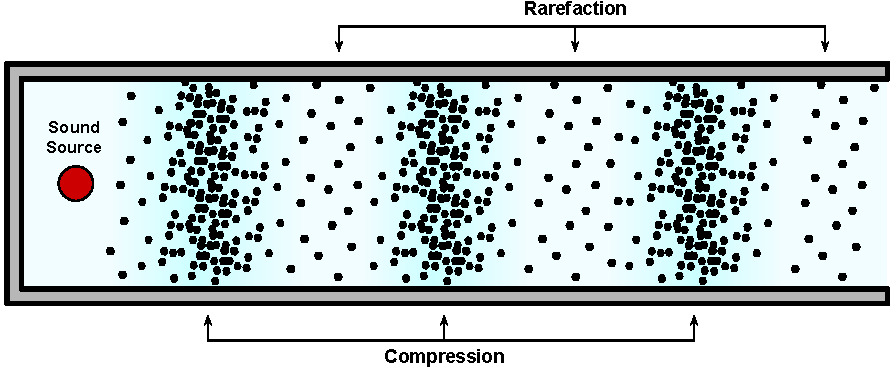
\includegraphics[width=0.65\textwidth]{figures/1Problem_analysis/Planar sound waves.pdf}
    \caption{Figure illustrating the principle behind propagation of sound in an open tube with fluid medium. Notice that different behaviours of sound, such as reflection, are ignored for simplicity. Adapted from \cite{Acoustics:Definition_of_sound1,Acoustics:Handbook_of_Acoustics}}
    \label{Sound:sound_propagation}
\end{figure}


Sound waves can be created by means of different processes, and knowledge of these would be beneficial during the solution's design phase to avoid unwanted sources of noise. A list of possible sound sources to be considered can be seen listed below. \cite{Acoustics:Handbook_of_Acoustics}

\begin{itemize}
    \item \textbf{Vibrating Bodies:} Objects that cause local air pressure to fluctuate through vibrations. An example of this could be an vibrating drumhead. 
    \item \textbf{Changing Airflow:} Any process that involves manipulation with air that causes a change in airflow. An example of this could be a human speaking. 
    \item \textbf{Time-Dependent Heat Sources:} A source that expands due to rapid heating. An example of this could be an explosion.     
    \item \textbf{Supersonic Flow:} Objects that cause air to move faster than sound, creating shock waves. An example of this could be a speeding bullet. 
\end{itemize}

%sometimes referred to as "pressure waves", and \cite{Acoustics:Definition_of_sound} 

% Sources of sound

% (Frequency, tone and amplitude)
    % Audible/inaudible (ultrasonic)

When discussing sound there is often distinguished between audible and inaudible sound. Audible sound is referring to sound which can be heard by the typical human being, and is in the frequency\footnote{Frequency is defined as vibrations per second or number of "waves" occurring each second. It denotes the pitch of the sound in this context \cite{Acoustics:Frequency_definition}.} range of 20 to 20.000 Hz. Inaudible sound is typically called either infra- or ultrasound. Infrasound denotes the frequencies below the audible frequency range (\<20 Hz) and ultrasound denotes the frequencies above it (\>20.000 Hz). This can be seen in Figure \ref{Sound:frequency_ranges}. \cite{Acoustics:Handbook_of_Acoustics,Acoustics:Neuroscience_Hearing_frequency}   

\begin{figure}[H]
    \centering
    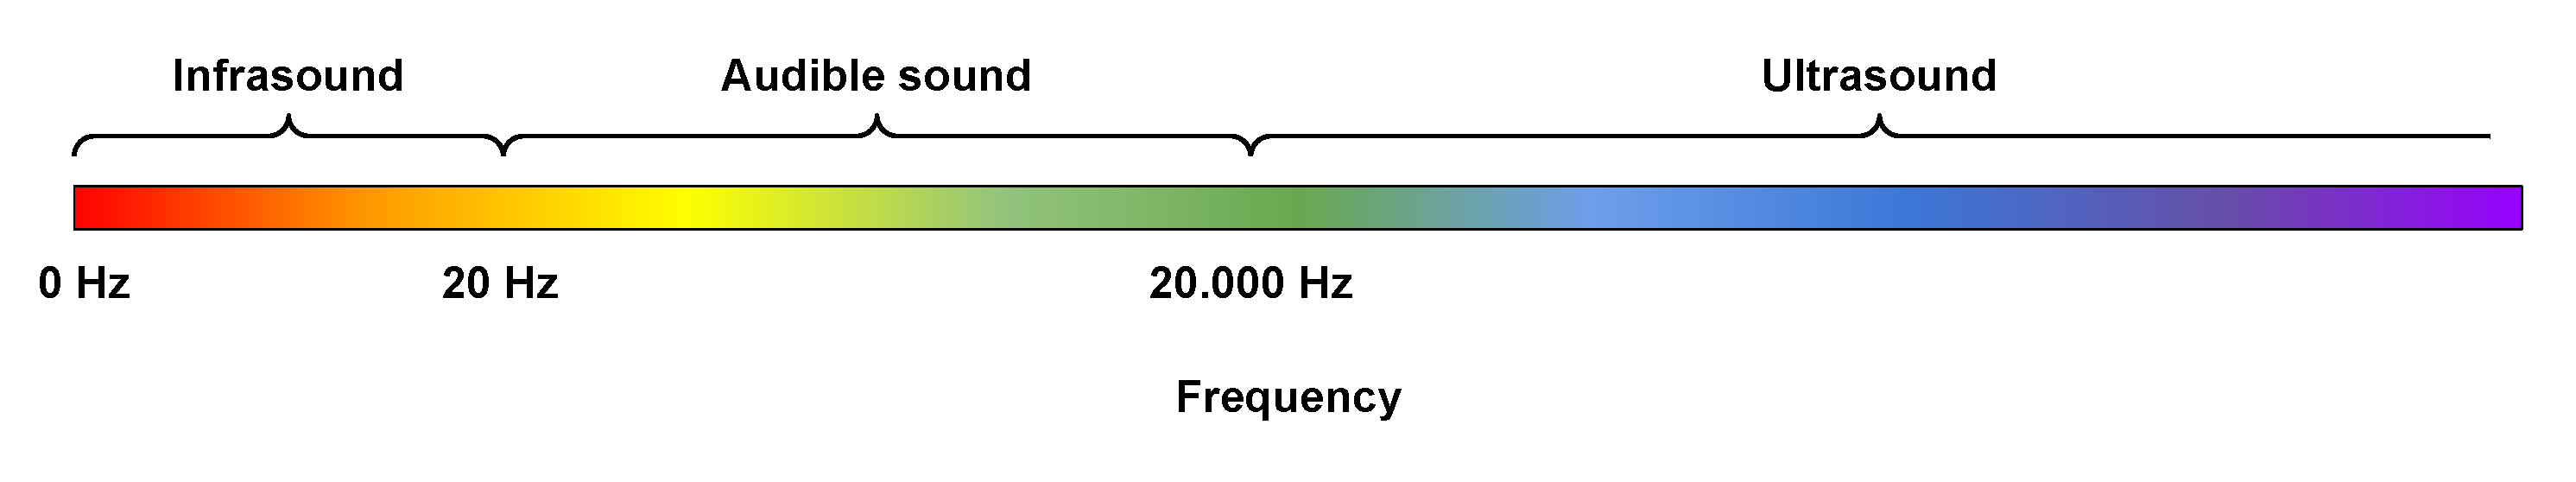
\includegraphics[width=1.05\textwidth]{figures/1Problem_analysis/Audible_and_inaudible_sound.pdf}
    \caption{Figure showing the frequency ranges of audible and inaudible sound.}
    \label{Sound:frequency_ranges}
\end{figure}

Even though inaudible sound cannot be captured physically by humans they can still be recorded and used by more sensitive equipment. Infrasound is used to detect natural occurrences such as earthquakes of volcanic eruptions, while ultrasound is used e.g. in medical science or as sonar underwater. \cite{Acoustics:Handbook_of_Acoustics}
%As both audible and inaudible sound can be used in many cases it is critical to understand how it is emitted and captured for it to be used in applications.  

Due to the available hardware, i.e. microphones and loudspeakers, this project will be dealing with sounds in the audible spectrum. Henceforth, the theoretical descriptions of hardware, with regard to sound, will be of the type made for audible sound.    

\subsubsection{Behaviour of Waves}
Sound waves exhibit different characteristics with respect to the propagation and interaction with mediums. To gain insight into these fundamental properties of sound waves, the topics \textit{reflection}, \textit{refraction}, \textit{diffraction}, and \textit{Inverse-square law} will briefly be covered.

The theory behind the first three properties will be supported by Figure \ref{fig:soundandmedium}, which illustrates a planar sound wave and flat surface.\footnote{Although the propagation of a sound wave is three-dimensional and propagates in all directions, it is convenient to represent the processes behind it as an idealised planar wavefront.\cite{Acoustics:Handbook_of_Acoustics}}.

\begin{figure}[H]
    \centering
    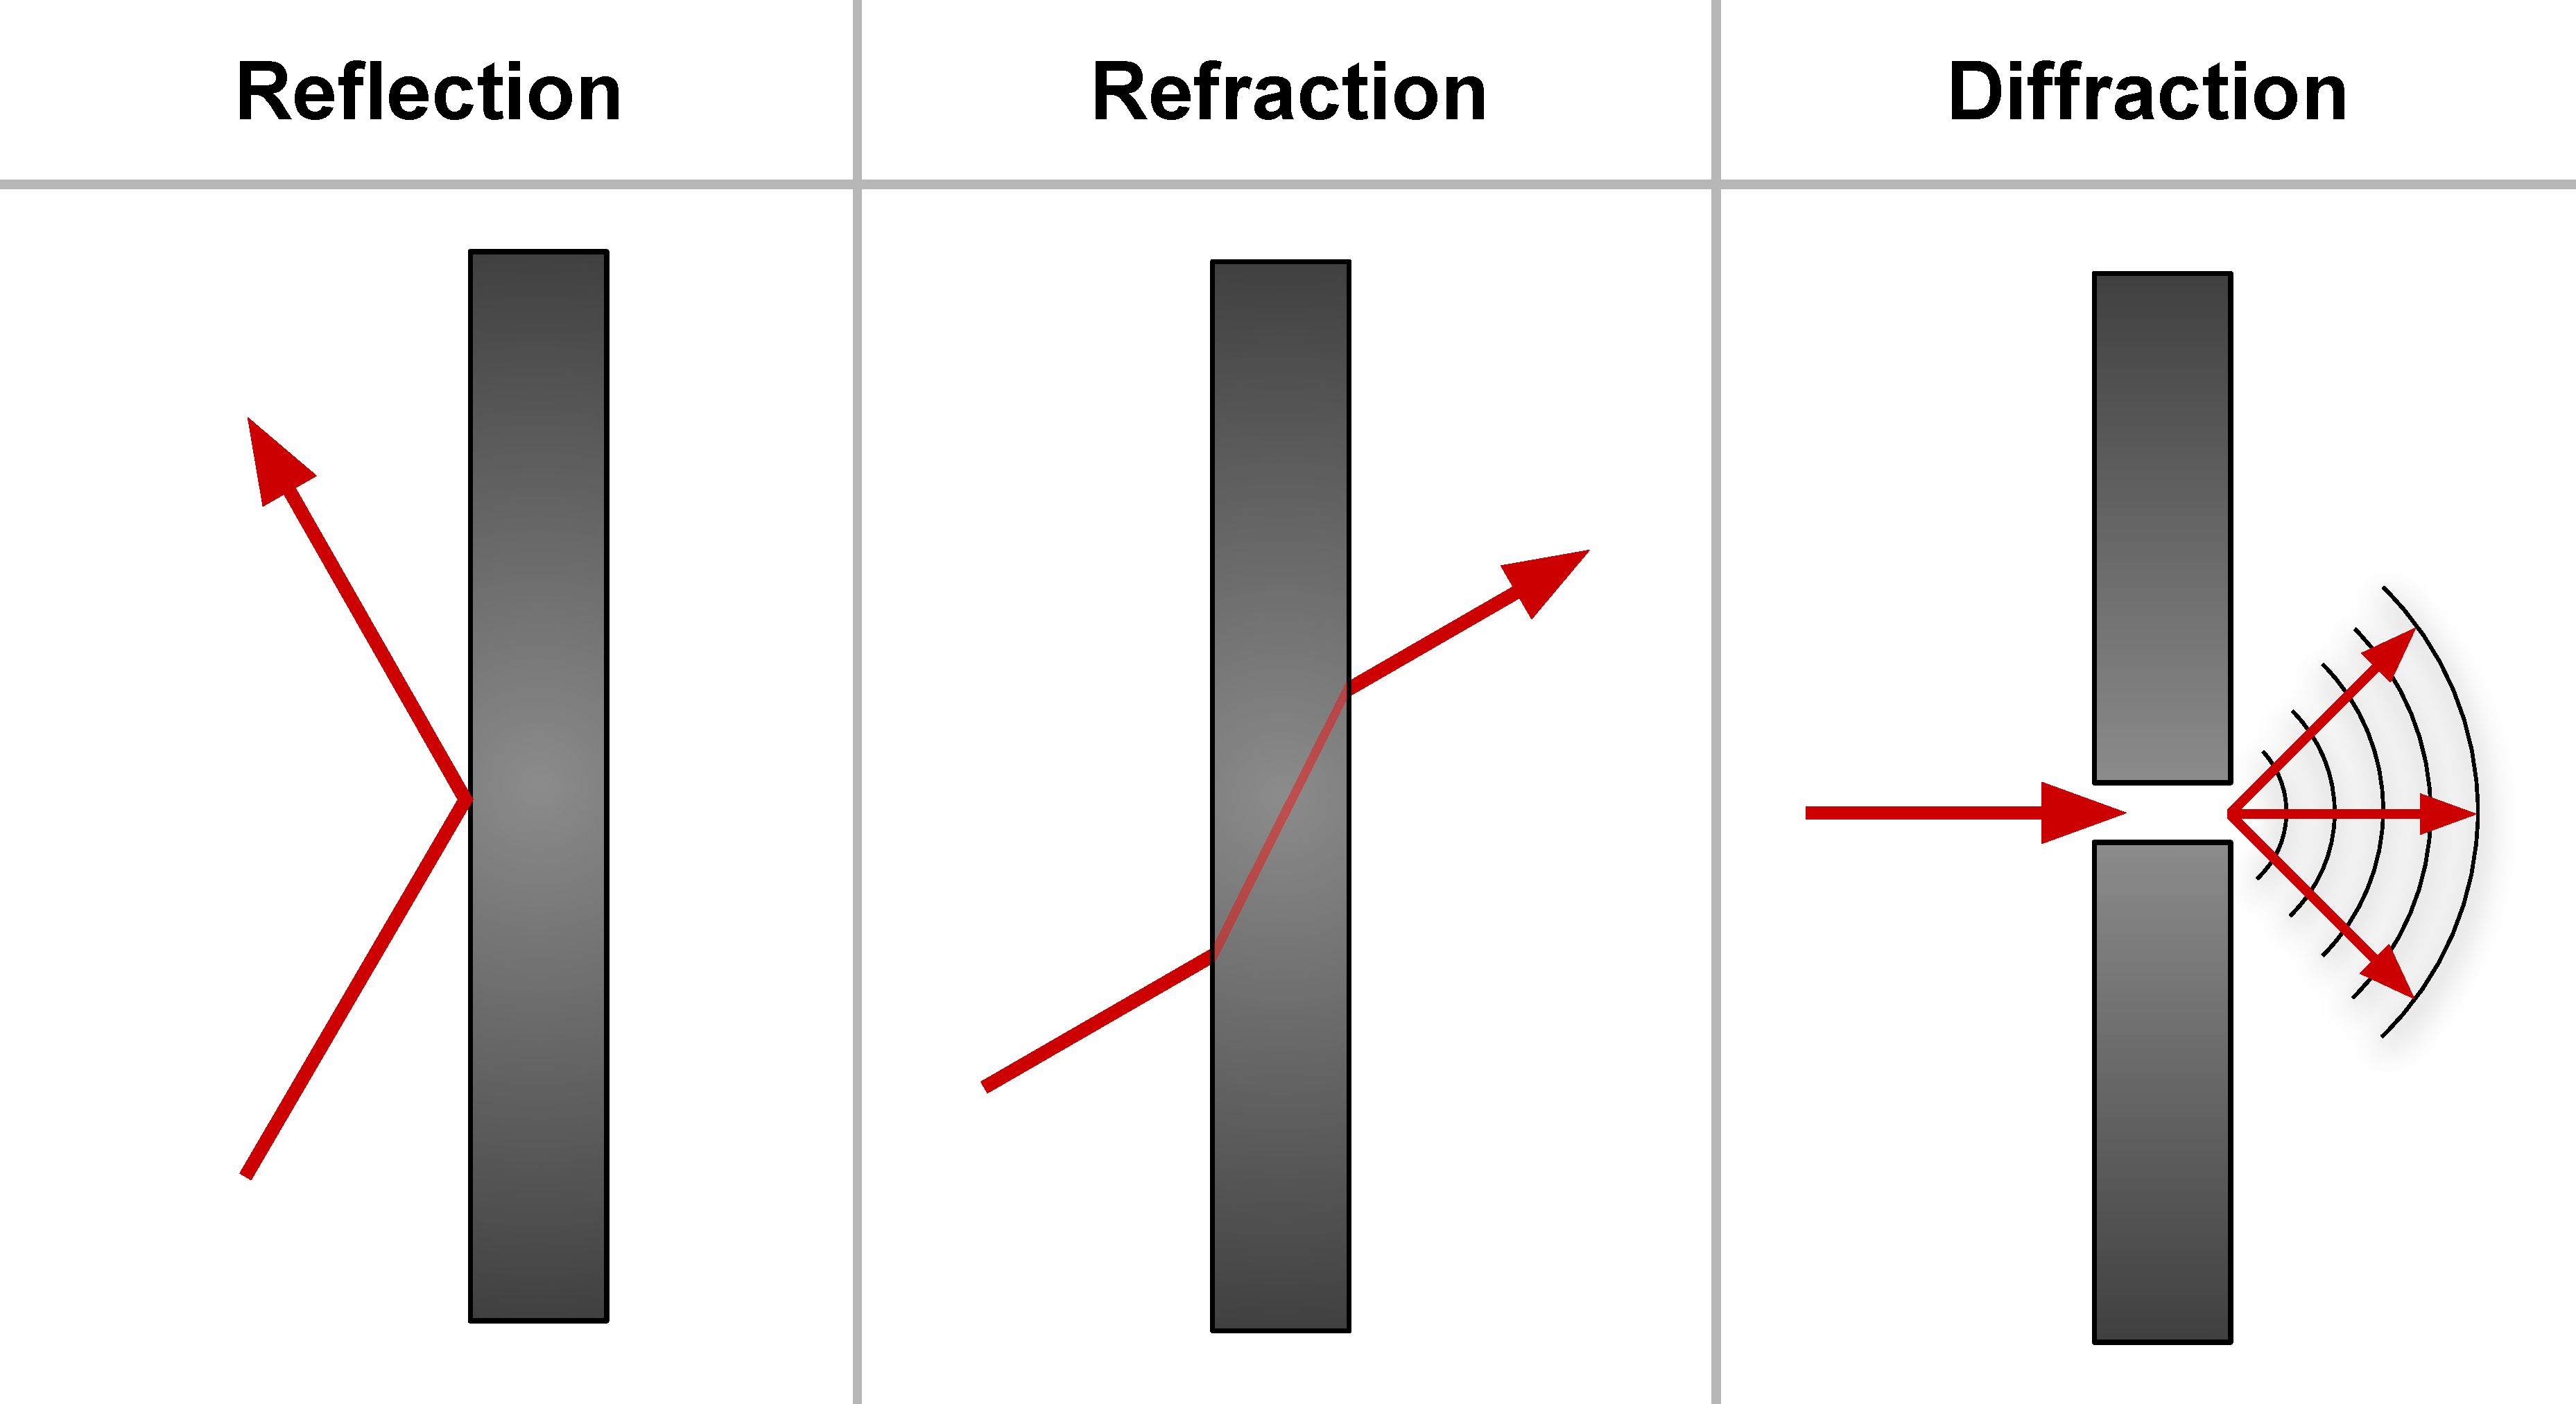
\includegraphics[width=0.8\textwidth]{figures/1Problem_analysis/Reflection_Refraction_Diffraction.pdf}
    \caption{Illustration of reflection, refraction, and diffraction.}
    \label{fig:soundandmedium}
\end{figure}

\textbf{Reflection}\\
When a planar sound wave reflects off a perfectly flat surface, as seen in the left of Figure \ref{fig:soundandmedium}, the angle of incidence will be equal to the angle of the outgoing reflection, regardless the angle of approach\footnote{A principle also known as the "\textit{law of mirrors}". \cite{Acoustics:Handbook_of_Acoustics}} \cite{Acoustics:Definition_of_sound3,Acoustics:Handbook_of_Acoustics}. Although this principle is introduced for flat surfaces, the law will also apply to ones that are curved; however, for these cases, the identical angles for the ingoing and outgoing ray will be measured with respect to the tangent at the point of incidence. 

\textbf{Refraction}\\
While reflection represents a change in direction by a sound wave impinging a surface, refraction is the change in direction caused by the transition between different mediums, as seen in the middle of Figure \ref{fig:soundandmedium}. A relation between the refraction, speed of sound, and medium is defined by Snell's law, as seen in Equation \ref{eq:SnellLaw}. \cite{Acoustics:Definition_of_sound3,Acoustics:Handbook_of_Acoustics} 

\begin{equation}\label{eq:SnellLaw}
    \frac{\sin{(\theta_2)}}{\sin{(\theta_1)}}\,=\,\frac{v_2}{v_1}\,=\,\frac{n_2}{n_1} 
\end{equation}

where $\theta_1$ and $\theta_2$ are the angles of incidence measured from the surface normal, $v_1$ and $v_2$ are the speeds of sound in the different mediums, and $n_1$ and $n_2$ are the refraction indexes for the two mediums. 

\textbf{Diffraction}\\
The phenomenon of diffraction is similar to both reflection and refraction, as it also represents a change in direction of a wave. However, diffraction occurs when sound is bent around an edge, as seen in the right of Figure \ref{fig:soundandmedium}\footnote{It is important to note that the figure is a simplification of diffraction. In reality, diffraction is the result of wave interference.\cite{Acoustics:Handbook_of_Acoustics}}. The degree to which sound is bent by this phenomenon can depend on the size of its wavelength relative to the size of the edge, and the shape of the wavefront that impinges the edge to cause diffraction. \cite{Acoustics:Handbook_of_Acoustics}

\textbf{Inverse-square law}\\
In relation to the propagation of sound waves, the inverse-square law states that the intensity per unit area is inversely proportional to the distance from the source. The intensity, $I$, is given as the power of the source, $P$, over the surface area of a sphere, as seen in Equation \eqref{eq:InvSquareLaw}
\begin{equation}\label{eq:InvSquareLaw}
    I = \frac{P}{4\,\pi\,r^2}
\end{equation}
where the radius, $r$, corresponds to the distance from the source. 

\textbf{Absorption}\\
When sound waves impinge a material, such as a wall or the ceiling, a quantity of the energy from the waves are lost when the sound is reflected; some transmitting through the material and some converted to heat. This causes an attenuation of the reflected sound intensity, which can be described by the absorption coefficient. The absorption coefficient, denoted $a$, is both dependant on the material and the frequency with which the sound waves propagate. It can be described by the proportion between the sound energy that is not reflected and the total sound energy, and as such $a\in[0,1]$. \cite{Acoustics:Absorption}

\textbf{Interaction between Waves}\\ 
When two or more waves encounter each other, a new wave is created as a result of their interaction. This result is the superposition of the two waves, which is simply obtained by taking the algebraic sum of the individual wave disturbances, as seen in Figure \ref{fig:superposition}.

\begin{figure}[H]
    \centering
    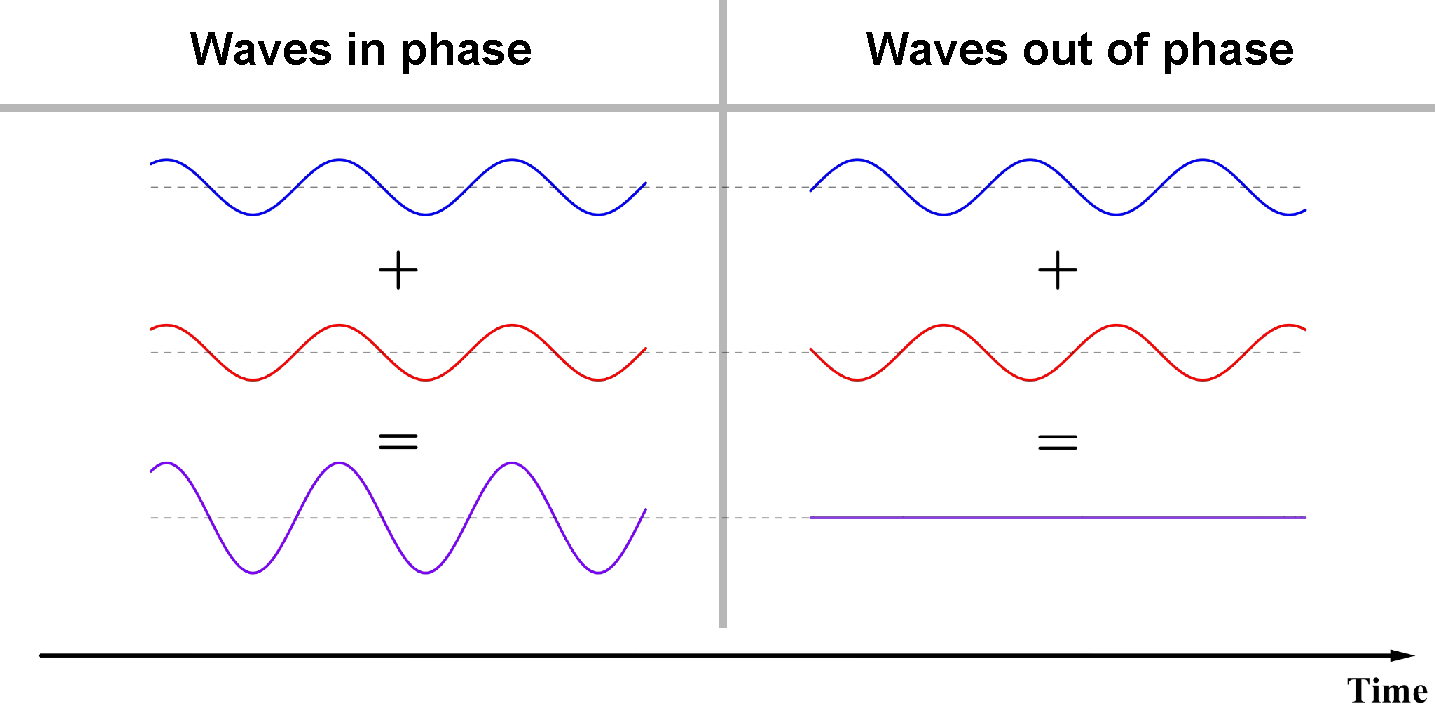
\includegraphics[width=0.8\textwidth]{figures/1Problem_analysis/Superposition.pdf}
    \caption{Superposition of two waves in phase (left) and two waves out of phase (right).}
    \label{fig:superposition}
\end{figure}

This can also be used to make speakers directive. By placing point sources at a given distance from each other, the pattern with which the sound is emitted, becomes directive. Depending on the amount of sources and distance between them, the pattern can be adjusted to the application. For a concentrated bidirectional beam, the distance between the point sources must be \nfrac{$\lambda$}{2}, with each adjacent source being out of phase with each other, whereas a distance of \nfrac{$\lambda$}{4} gives a unidirectional beam.

\textbf{Waves in a Closed Room}\\
In a situation with a person that talks to a listener in a closed echoic room, the sound will not only travel the direct path to the listeners ears. It will also travel through the entire room, bouncing off any surfaces it encounters to then be heard by the listener. This is due to the phenomenon of echoes, which is simply reflected sound waves reaching a listener. After a sound has been made, these reflections multiply rapidly until an infinitude of sound reflections envelop the entire room, known as reverberation. The scenario can be seen on the left of Figure \ref{fig:direct_early_reverb}.

\begin{figure}[H]
    \centering
    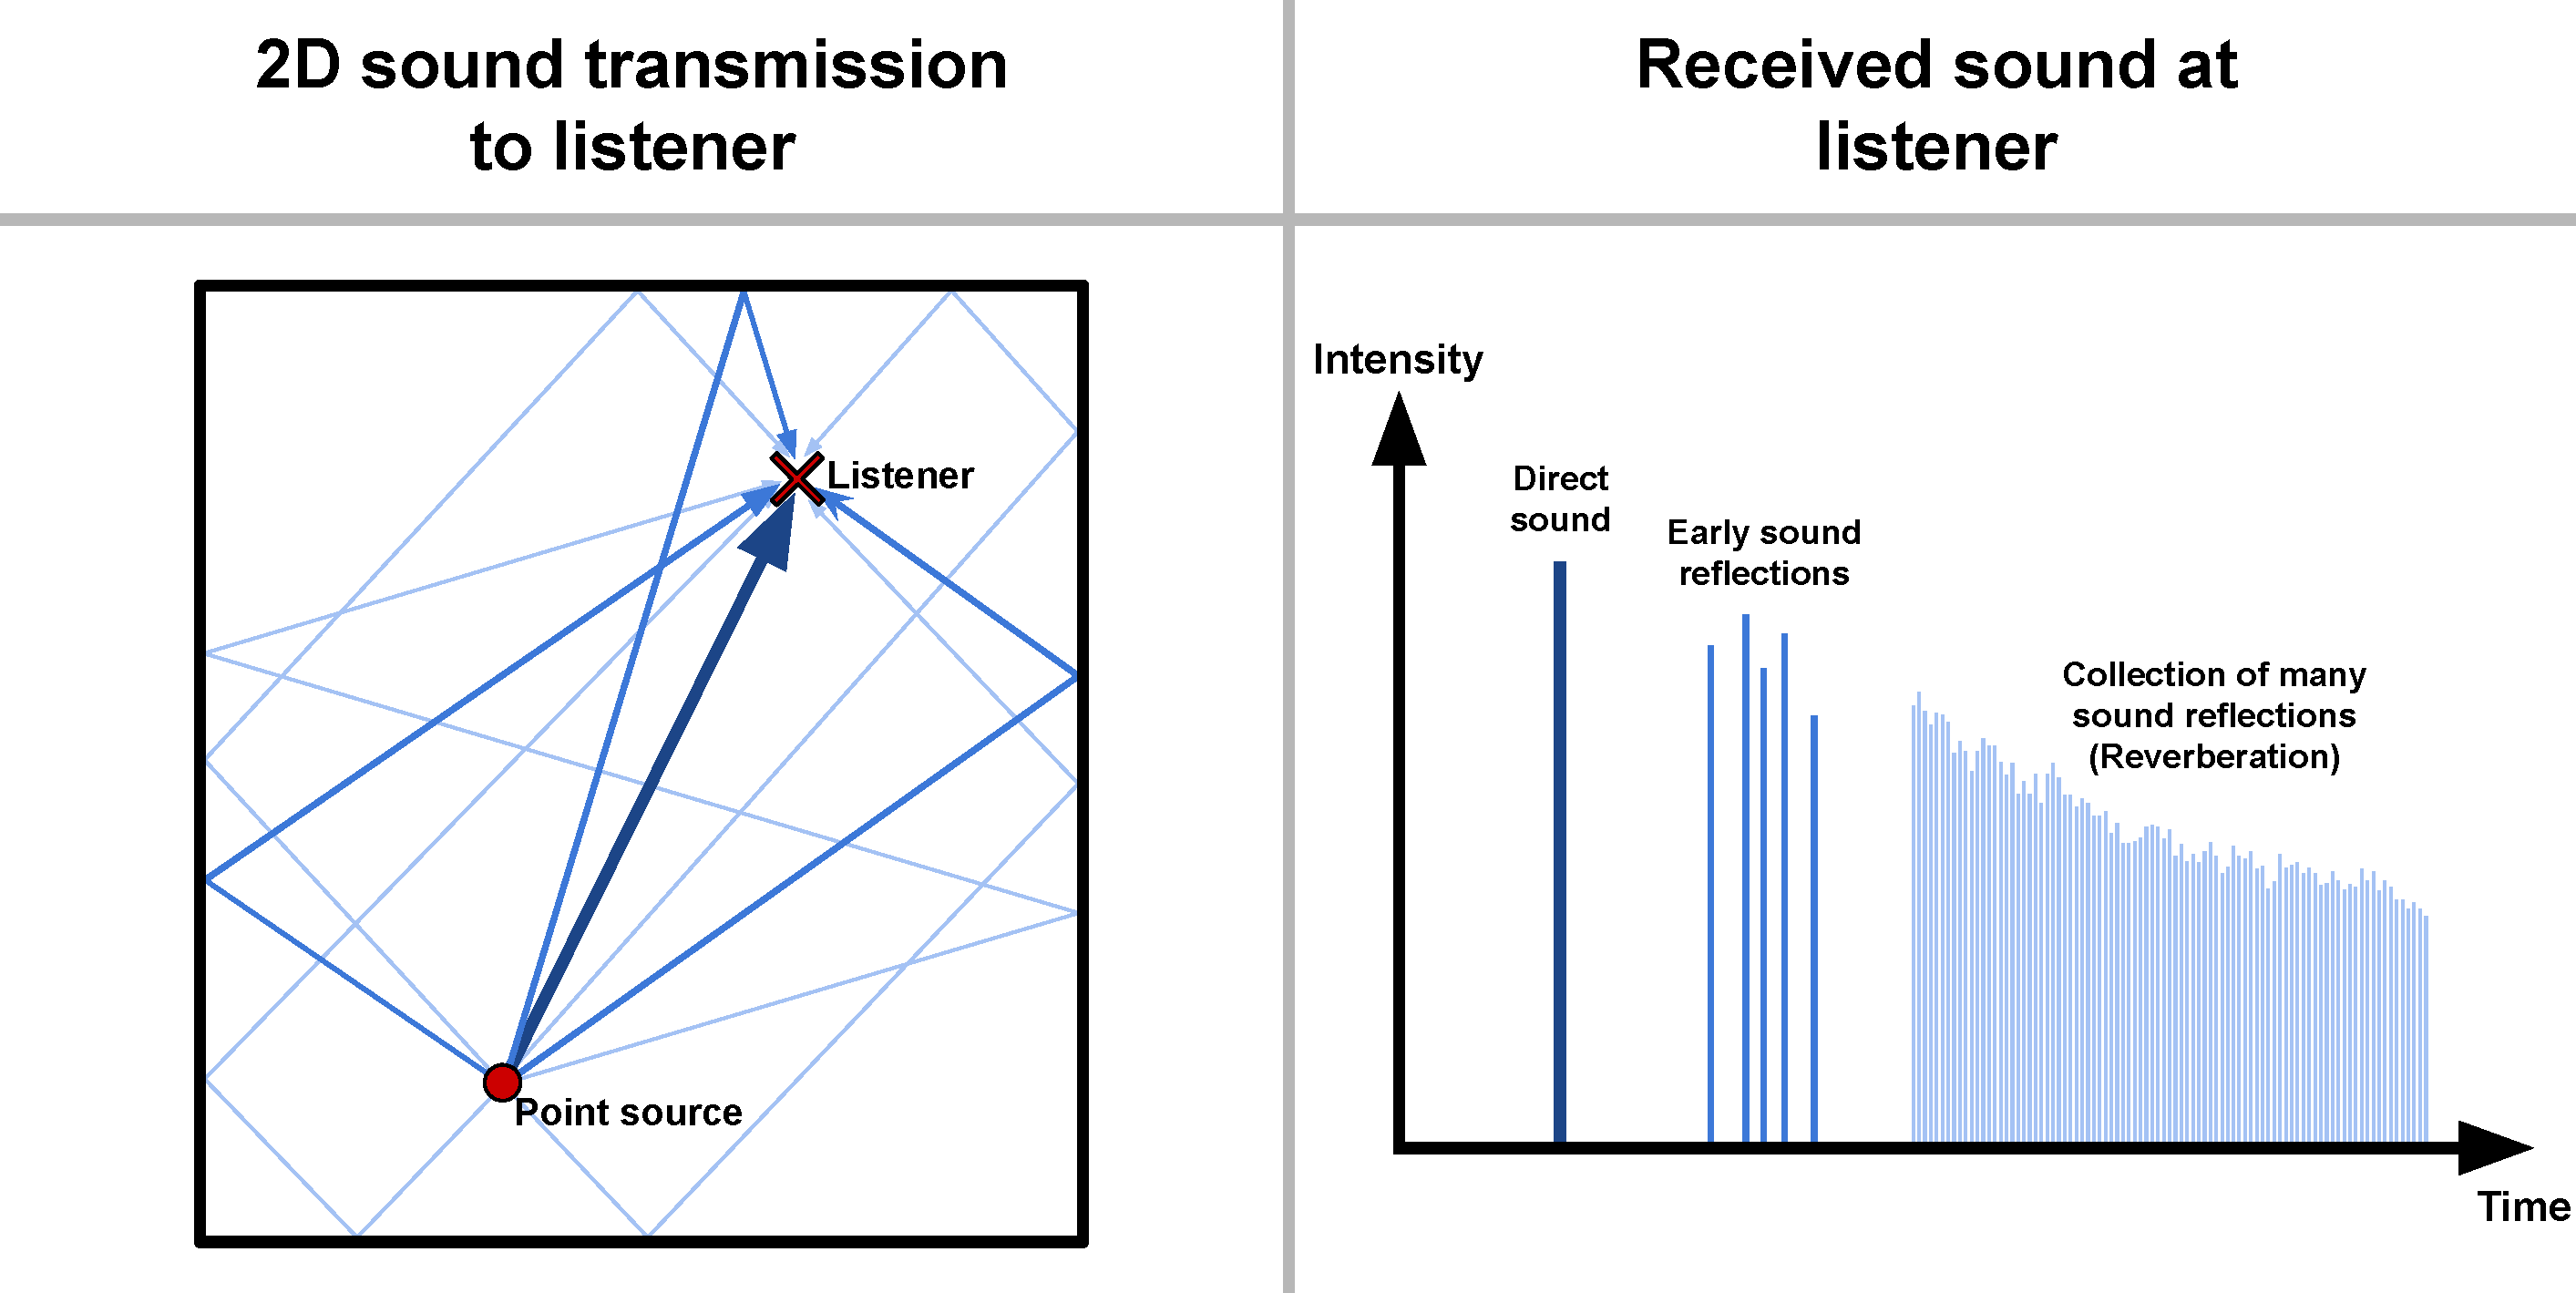
\includegraphics[width=\textwidth]{figures/1Problem_analysis/Reverb_early_direct.pdf}
    \caption{Propagation of sound in a closed room with a point source and a listener, consisting of the direct sound, early reflections, and a multitude of later reflections (reverberation). \textit{Left:} The two dimensional depiction of the transmission of sound. \textit{Right:} The graphical depiction of the transmission of sound containing intensity over time (room impulse response).}
    \label{fig:direct_early_reverb}
\end{figure}

Due to the inverse-square law and absorption, as time passes and more reflections occur, the energy of the sound waves gradually dissipate. This can be seen in the graph on the right of Figure \ref{fig:direct_early_reverb}, where the intensity of the sound waves reaching the listener is plotted as a function of time, given an initial sound impulse from the point source. It can be seen, that while the energy is generally decreasing as time goes, there is still some stochastic behaviour. Furthermore, the number of reflections of the sound waves can be distinguished from the time of arrival in the three categories represented on the graph.

\subsection{Robotic Sensors}\label{subsec:RoboticSensors}
When a robot needs to perceive the environment to give an idea of how to react in certain situations, it is imperative that the robot must first obtain data from the real world. This is achieved with the application of a series of sensors on the robot, with the number and type being chosen with respect to the specific application. For mapping an unknown environment, at least two sensors are required; one for measuring the obstacles and objects in the environment, and one for measuring the location of the robot itself.


%In terms of sound, transducers\footnote{Transducers are devices that convert some form of energy. This could be a physical signal which is captured by the transducer and then converted into an electrical signal. \cite{Acoustics:Audio_production}} could be loudspeakers and microphones, which are used to emit and capture sound. These transducers allow sound waves to be either created from electrical signals or read and then converted into electrical signals. \cite{Acoustics:Audio_production}

\subsubsection{Microphones}
The microphone is the device that captures sound waves and converts it into electrical signals, which can then be processed. Multiple variations of the microphone exist each with their own advantages and disadvantages. Therefore it is of importance to select the type of microphone with respect to the intended use and the environment. \cite{Acoustics:Audio_production}

\textbf{Dynamic microphones} or \textbf{pressure microphones} are constructed with a thin diaphragm, a voice coil and a magnet. The diaphragm reacts with incoming sound waves, which causes it to move. The added pressure causes the voice coil to move. As this coil sits within the magnetic field of a magnet, the movement of the coil will cause changes in the magnetic field which induces an electric current into the voice coil. This current can be captured and is the audio signal. The functional principles of this type of microphone can be seen in Figure \ref{fig:dynamic_microphone}. \cite{Acoustics:Audio_production} 

\begin{figure}[H]
    \centering
    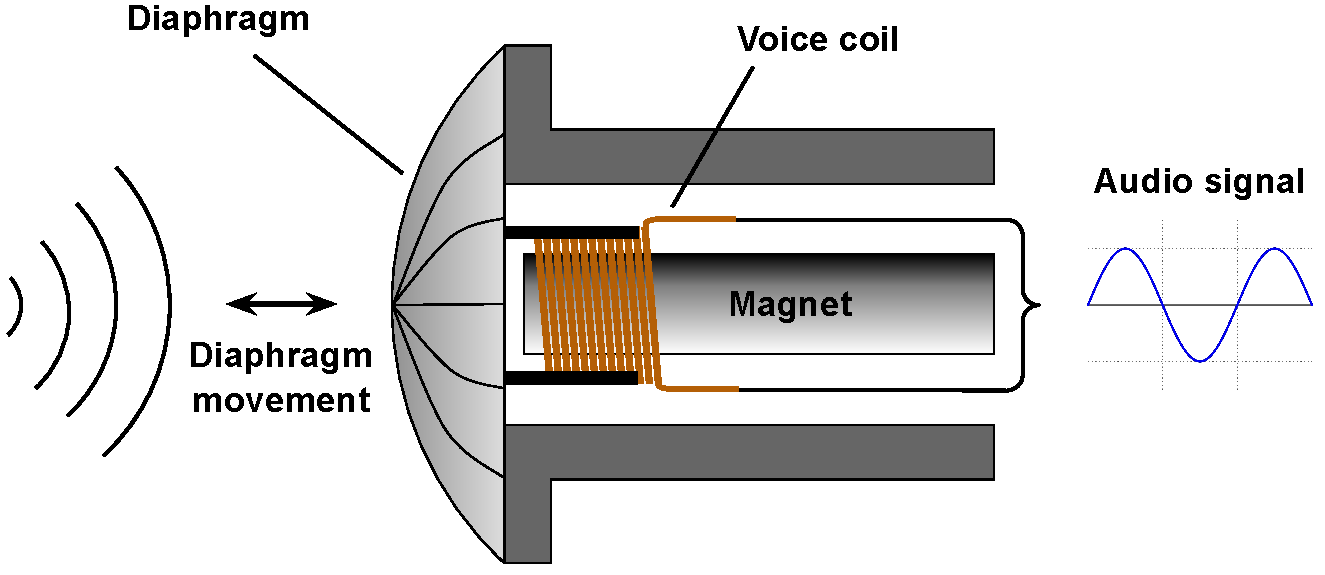
\includegraphics[width=0.9\textwidth]{figures/1Problem_analysis/Dynamic_microphone.pdf}
    \caption{Dynamic microphone showing some of the internal components such as the diaphragm, voice coil and magnet. Adapted from \cite{Acoustics:Audio_production, Acoustics:Jespers_slides}.}
    \label{fig:dynamic_microphone}
\end{figure}

\textbf{Condenser microphones} uses a capacitor to convert sound waves into electrical signals. These consists of a charged conductive diaphragm and a charged backplate. Spacing between these two components creates a space of air which functions as a capacitor. As the diaphragm reacts to sound waves the spacing between it and the backplate changes. This causes a change in the capacitance, which provides an electrical current. This electrical current translates to the audio signal. A condenser microphone typically contain an amplifier which amplifies the electrical signal as it can be hard to read. The functional principles of this type of microphone can be seen in Figure \ref{fig:condenser_microphone}.\cite{Acoustics:Audio_production} 

\begin{figure}[H]
    \centering
    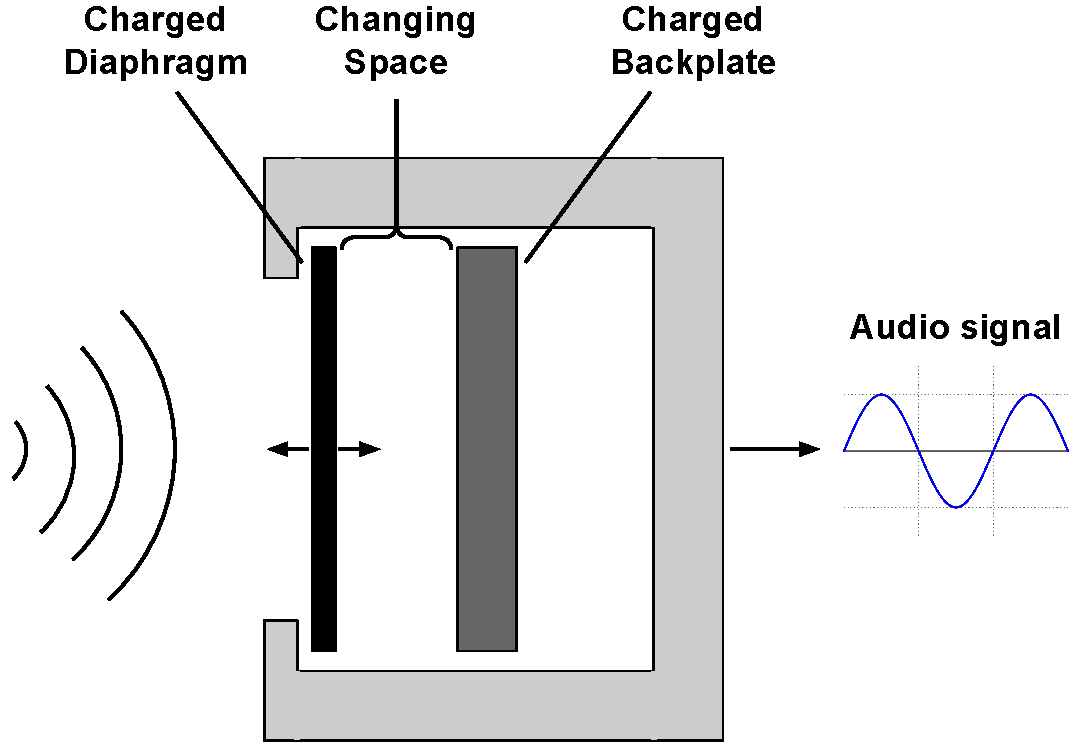
\includegraphics[width=0.8\textwidth]{figures/1Problem_analysis/condenser_microphone.pdf}
    \caption{Condenser microphone showing some of the internal components such as the charged diaphragm and the charged backplate. Adapted from \cite{Acoustics:Audio_production}.}
    \label{fig:condenser_microphone}
\end{figure}

\textbf{Ribbon microphones} uses a metal ribbon diaphragm, which is situated between the poles of a magnet. The ribbon reacts to incoming sound waves and moves. This movement causes a change in the magnetic field, which can be captured as an electric current. This can be translated into the audio signal. The functional principles of this type of microphone can be seen in Figure \ref{fig:Ribbon_microphone}. \cite{Acoustics_book_on_ribbon_microphone}

\begin{figure}[H]
    \centering
    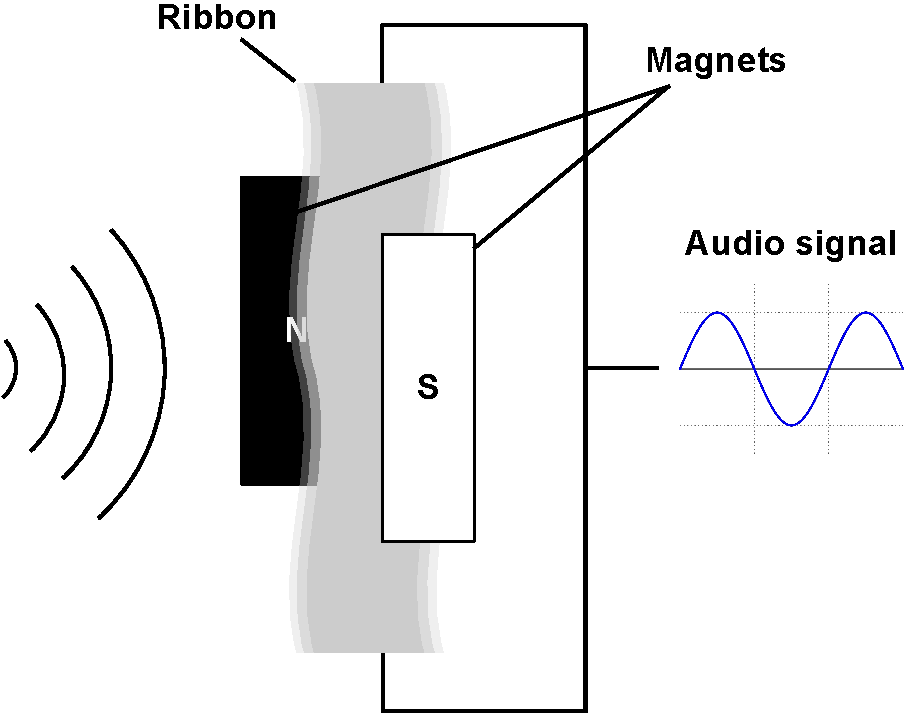
\includegraphics[width=0.8\textwidth]{figures/1Problem_analysis/Ribbon_microphone.pdf}
    \caption{Ribbon microphone showing some of the internal components such as the ribbon and the magnets. Adapted from \cite{Acoustics_book_on_ribbon_microphone}.}
    \label{fig:Ribbon_microphone}
\end{figure}

Multiple other microphone variations exist, however the dynamic, condenser and ribbon microphones are deemed the main types, and other variations will therefore not be covered. \cite{Acoustics_book_on_ribbon_microphone}

The different microphone types are summarised in Table \ref{tab:microphone_types} along with advantages and disadvantages. 

\begin{table}[H]
    \centering
    \begin{tabular}{?M{2.5cm}?M{4.4cm}|M{4.4cm}|M{4.4cm}?} \boldline
         & Dynamic & Condenser & Ribbon  \\\boldline
        Conversion & \raisebox{-1mm}{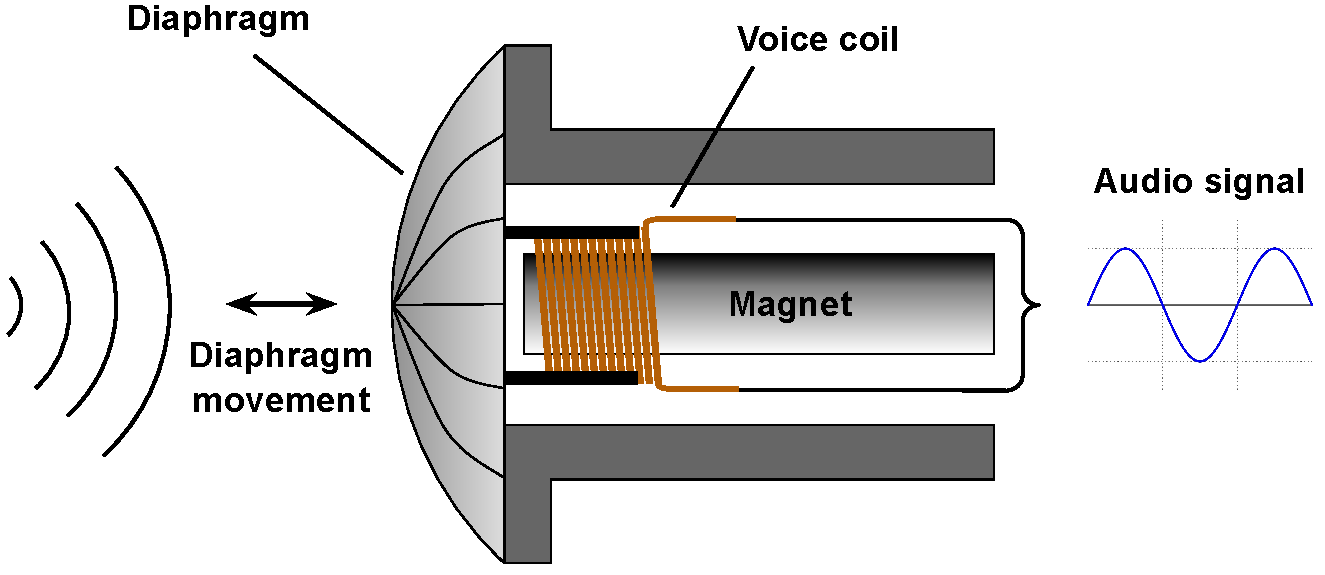
\includegraphics[width=0.26\textwidth]{figures/1Problem_analysis/Dynamic_microphone.pdf}} & \raisebox{-1mm}{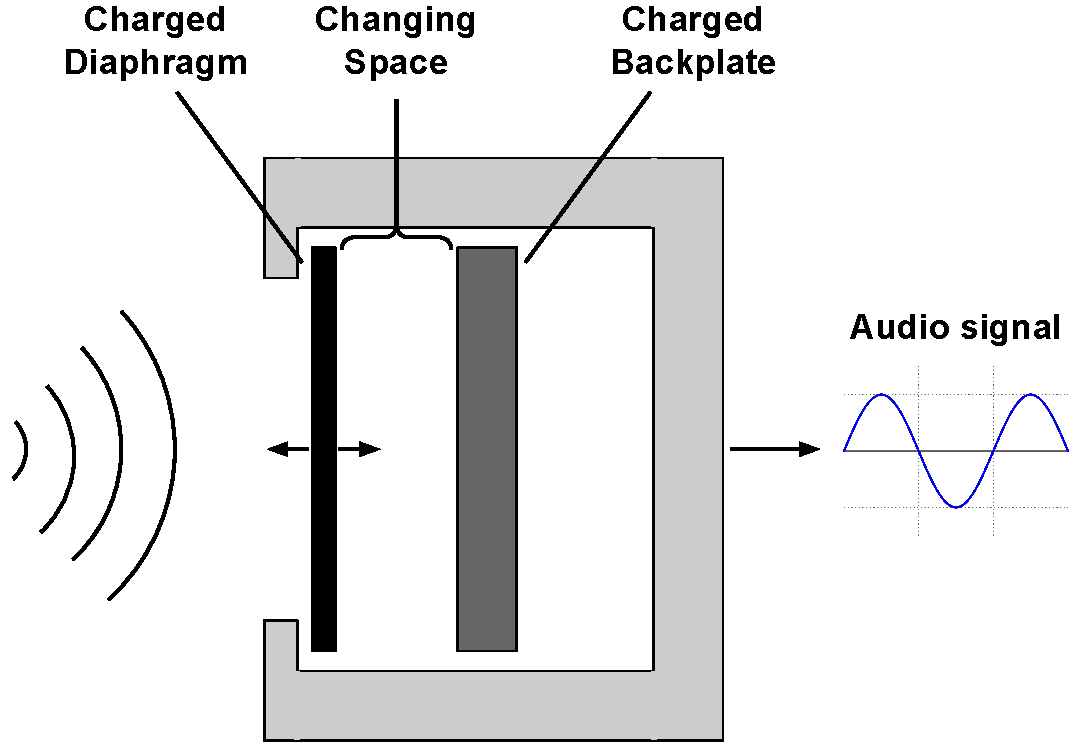
\includegraphics[width=0.26\textwidth]{figures/1Problem_analysis/condenser_microphone.pdf}} & \raisebox{-1mm}{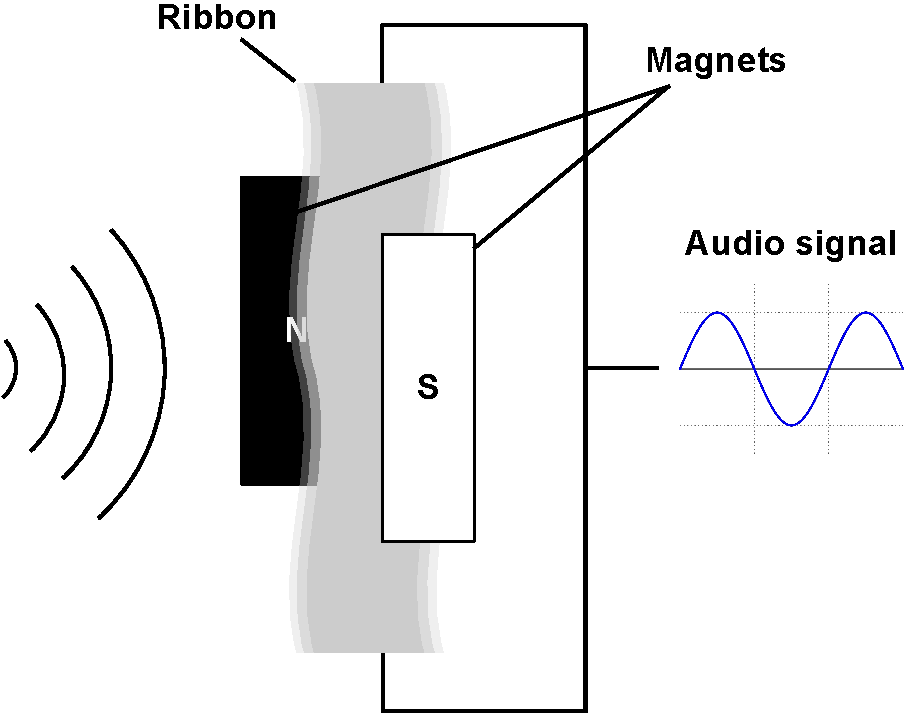
\includegraphics[width=0.26\textwidth]{figures/1Problem_analysis/Ribbon_microphone.pdf}}  \\\hline
        Application & General use, studio & Studio & Radio, Live performances  \\\hline
        Advantages & Great frequency response, sturdy & Great transient response, great frequency response & Accurate sound capture, low noise   \\\hline
        Disadvantages & Low level sounds can be missed & Self-generated noise can occur & Fragile, Sensitive, Expensive  \\\boldline
    \end{tabular}
    \caption{Showing the three main types of microphones along with usual applications, advantages, and disadvantages.\cite{Acoustics_book_on_ribbon_microphone, Acoustics:Audio_production}}
    \label{tab:microphone_types}
\end{table}

%%%%%%%%%Hvad gør jeg lige med sections her? (Spørg de andre)%%%%%%%%%%%%%%
\textbf{Pickup patterns} indicates the spectrum of which a microphone can detect sound. This varies from microphone to microphone and allows further differentiation between microphones besides the way it converts sound waves into electrical signals.

The general pickup patterns are \textbf{omnidirectional}, \textbf{cardiod} or \textbf{bidirectional}, which refers to the direction or spectrum in which the microphone can capture sound. The \textbf{omnidirectional} pickup pattern is capable of capturing sound from all directions. This type of microphone is preferable when it is needed to capture sound from all directions. The \textbf{cardiod} pickup pattern is often further sub-categorised with respect to the pattern of its capturable spectrum. This type is intended to capture sound from one direction, the side of the microphone and to a small degree, behind the microphone. The \textbf{bidrectional} pickup pattern is capable of capturing sound from the front and the back of the microphone equally well. It is however not built to capture sound from the sides. The pickup pattern of certain microphones should be considered as the properties varies and therefore applicability to different sound capturing situation. The advantages and disadvantages can be seen in Table \ref{tab:Pick_up_patterns}. \cite{Acoustics:Audio_production}

\begin{table}[H]
    \centering
    \begin{tabular}{?M{2.5cm}?M{4.4cm}|M{4.4cm}|M{4.4cm}?} \boldline
         & Omnidirectional & Cardioid & Bidirectional  \\\boldline
        Pickup Pattern & \raisebox{-1mm}{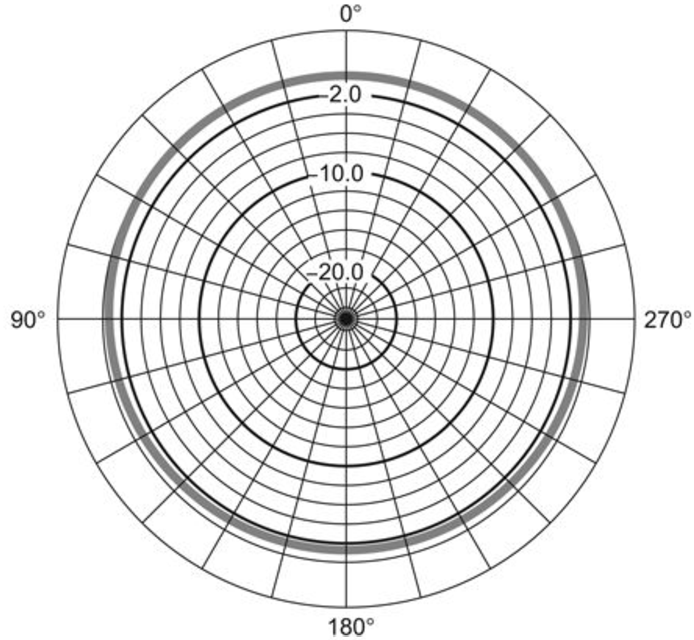
\includegraphics[width=0.26\textwidth]{figures/1Problem_analysis/Omnidirectional.pdf}} & \raisebox{-1mm}{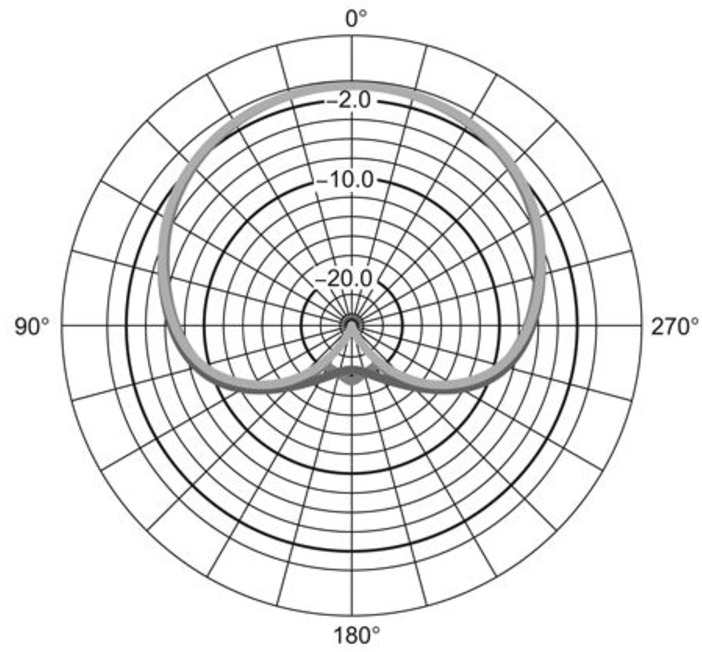
\includegraphics[width=0.26\textwidth]{figures/1Problem_analysis/Cardioid.pdf}} & \raisebox{-1mm}{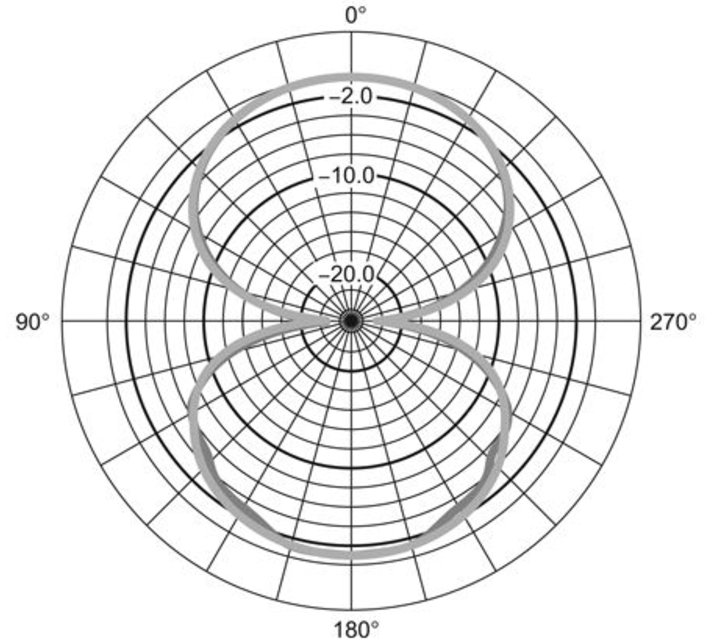
\includegraphics[width=0.26\textwidth]{figures/1Problem_analysis/Bidirectional.pdf}}  \\\hline
        Advantages & Capable of detecting sounds from all directions & Rejects unwanted sounds from other directions & Front and back of the microphone can be captured  \\\hline
        Disadvantages & Captures unwanted background noise & Accidentally moving "off-axis" & Not often applicable  \\\boldline
    \end{tabular}
    \caption{Showing the three main types of pickup patterns. Figures taken from \cite{Acoustics:Audio_production}.}
    \label{tab:Pick_up_patterns}
\end{table}

%%%%%%%%%%%%%%%%Overvej at slet dette afsnit%%%%%%%%%%%%%%%%%%%%%%%%
\textbf{Ultrasound microphones} are capable of detecting inaudible sound meaning sounds with a frequency above 20.000 kHz, as seen in Figure \ref{Sound:frequency_ranges}. Due to the higher frequency; ultrasound waves have a shorter wavelength, which is more precise, in terms of echolocation, than longer wavelengths. This is due to the principles of diffraction and reflection. If the wavelengths are bigger the occurrence of diffraction is higher, thus the sound travels in other directions. However, if the wavelengths are smaller more reflection will occur, and more precise capturing of the objects and environment will be present. \cite{Acoustics:Definition_of_sound3}     
%%%%%%%%%%%%%%%%%%%%%%%%%%%%%%%%%%%%%%%%%%%%%%%%%%%%%%%%%%%%%%%%%%%%


\subsubsection{Microphone Arrays}
Microphone arrays are comprised of several microphones arranged in a specified configuration to capture sound from different points in space, enabling more in-depth perception of the environment. With only one microphone, it is very difficult and imprecise to estimate directions, but with several microphones, placed with a known position relative to each other, the problem reduces to mathematical calculations related to the geometry of the setup. This is however with the assumption that the signal is static throughout the room, meaning the retrieved signal does not change between the microphones. Using several microphones and making assumptions about the propagation of the sound, one can use the time difference of arrival (\gls{TDOA}) to estimate the direction that a sound is coming from. Furthermore, the microphone array can be used as a beamformer, i.e. only allow sound to arrive from a specific direction at a time, also by utilising the \gls{TDOA}s between microphones. 

Overall, there are three parameters to the setup of the microphone array that must be determined. These are the shape of the array, the number of microphones, and the distance between the microphones. Starting with the shape, there are several ways to configure the microphones, e.g. a linear array, a circular array, or a spherical array. Comparing the three mentioned, the linear array is the simplest, while the spherical array is the most complex. This is due to how many dimensions the microphone array spans. The linear array can measure direction in 2D, but has an ambiguity considering backwards and forwards; the circular array can fully measure direction in 2D, but has an ambiguity between downwards and upwards when advancing to 3D; and the spherical array can fully measure direction in all three dimensions. When having decided the shape of the array, the number of microphones must be established. It could be anywhere between the minimum of two and however many one would desire. Generally, the more microphones there are in the array, the better representation of the sound source can be achieved, but this also comes with the obvious trade-off that more data needs to be processed. Often, between two and eight microphones are used for planar arrays. Knowing both the shape and number of microphones, the relative distances of the microphones is an important factor. Almost for all microphone arrays, the microphones are placed at equidistant length from each other for apparent simplification purposes. Therefore, only one distance must be determined, which relates to the size of the array. A larger distance, will correspond to an array with a larger area, and vice versa. Additionally, if the microphones are far apart, it is more likely that the signal captured in each microphone is different, because of the longer travel time between them. This could then result in less accurate readings and consequently \gls{TDOA}s. However, if the microphones are very close to each other, it will be difficult to distinguish between the \gls{TOA}s in each microphone. This shorter distance also causes the resolution to decrease, because the signal is sampled, meaning a finite lowest possible value. To compensate for the loss of resolution, the sampling rate would then have to be increased. \cite{Acoustics:Handbook_of_Acoustics}
% very far: more noise, less accurate
% very close: too close readings, lower resolution
% sweetspot

\begin{figure}[H]
    \centering
    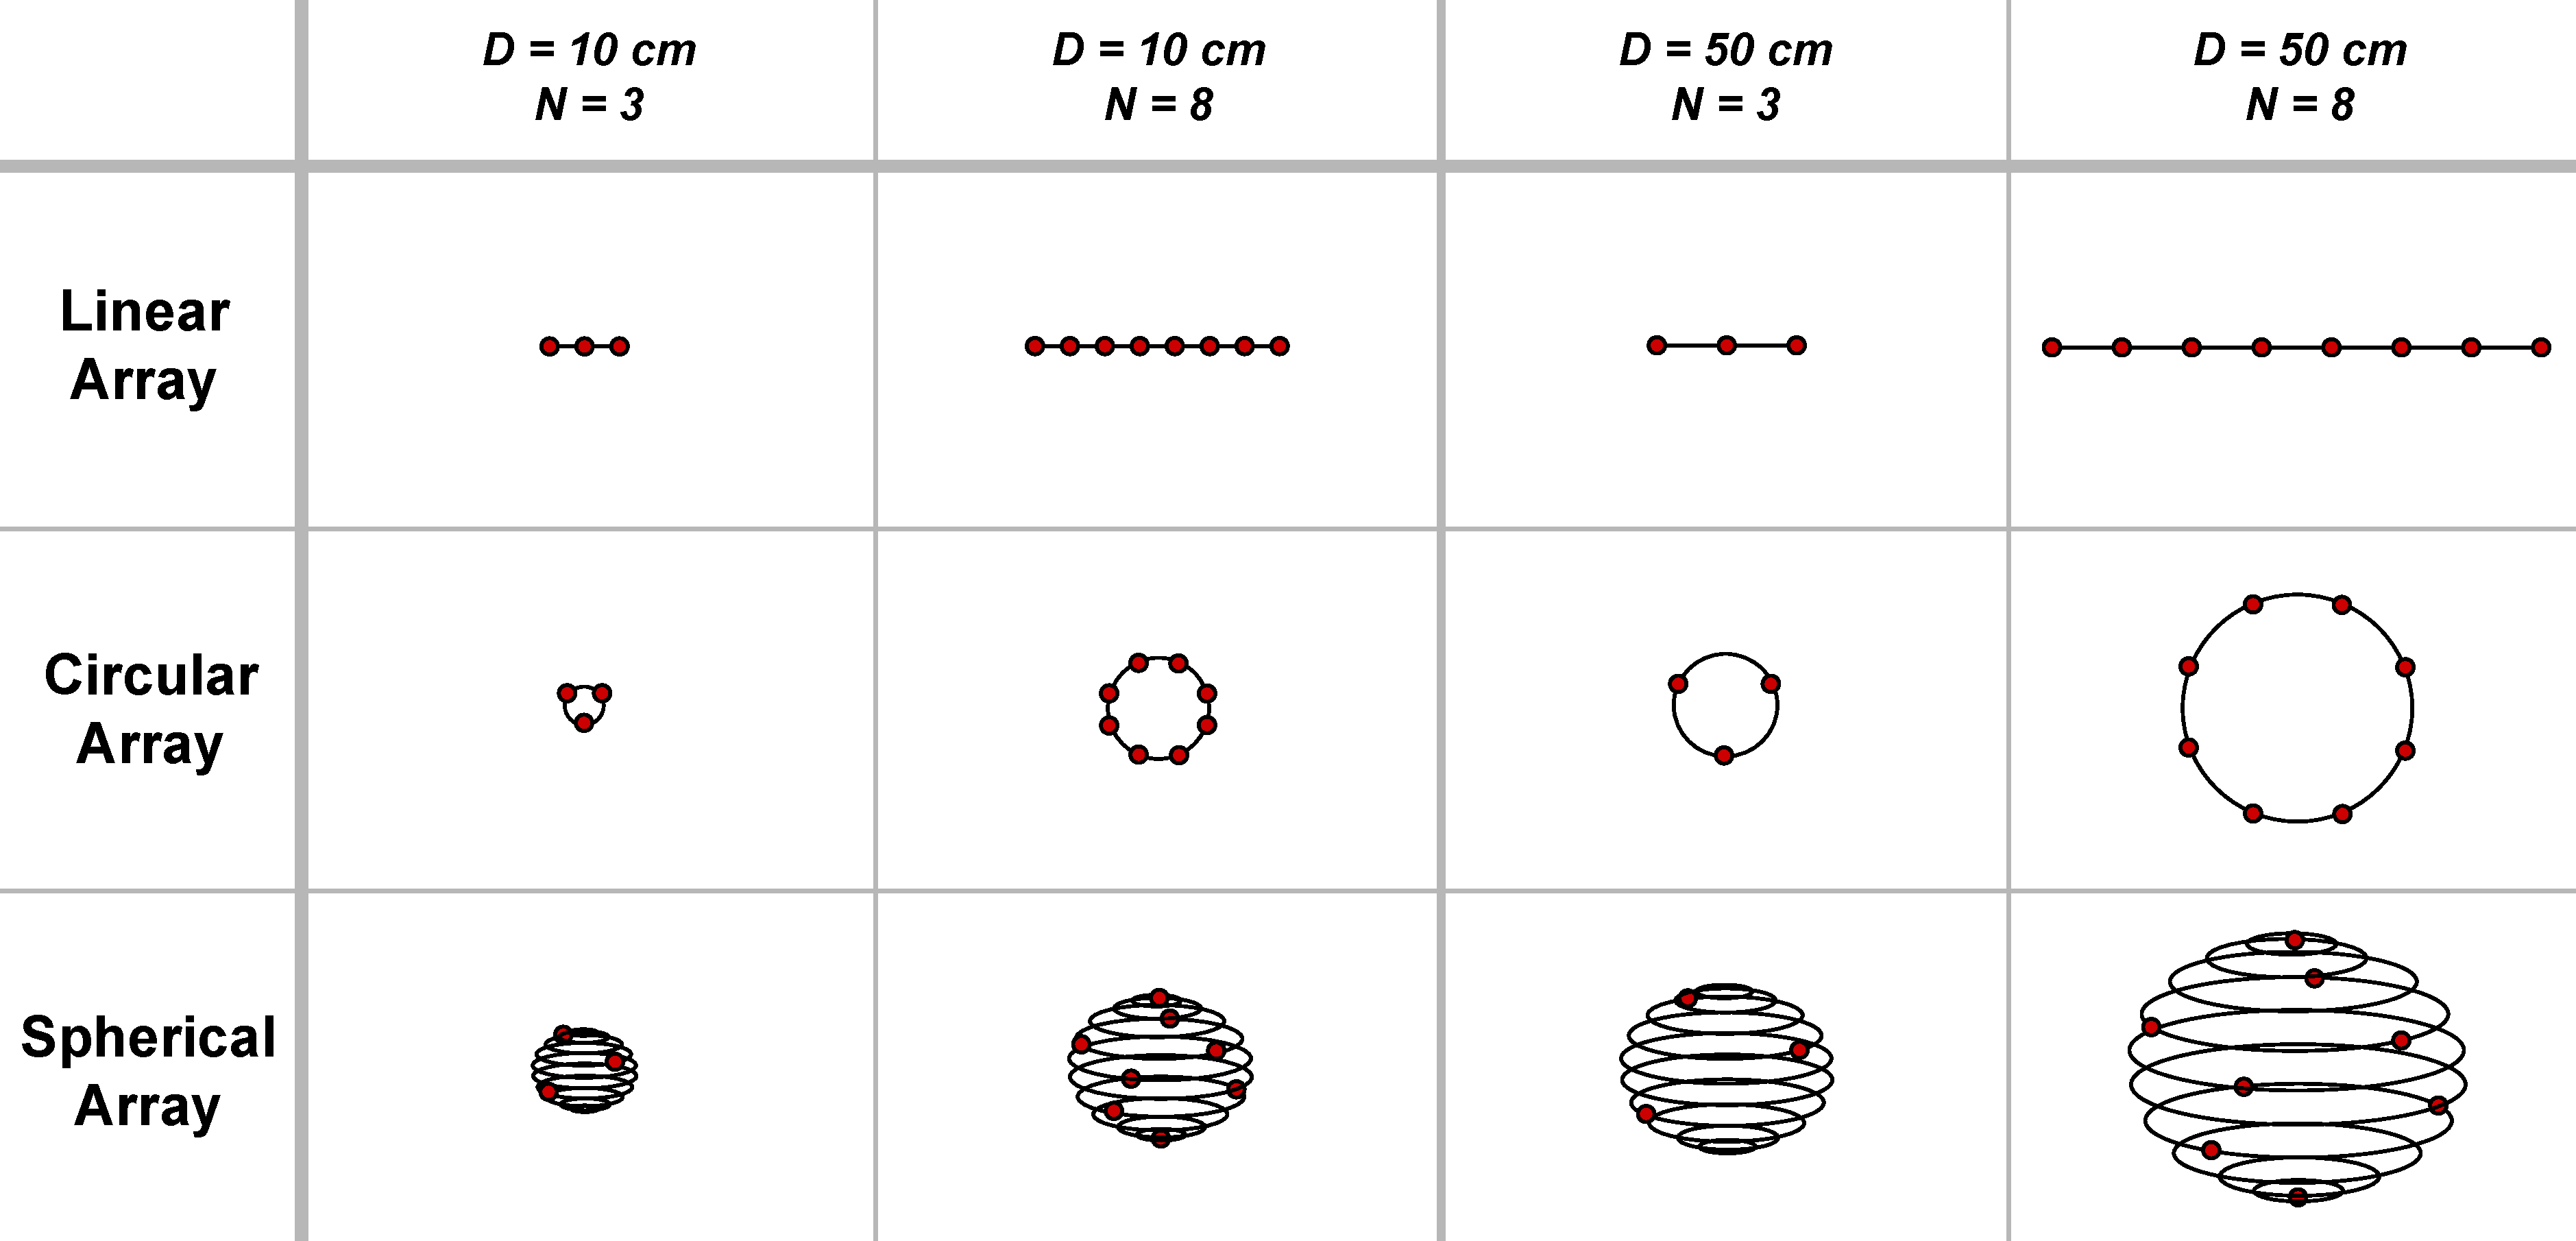
\includegraphics[width=\textwidth]{figures/1Problem_analysis/Microphone_array.pdf}
    \caption{Illustration of different microphone array combinations, with the different parameters \textit{type}, \textit{distance}, and \textit{number}. The symbols in the top row are distance ($D$) and number of microphones ($N$).}
    \label{fig:mic_array}
\end{figure}

\subsubsection{Odometry Sensors}
Odometry is a widely used approach of determining a mobile robot's position and orientation relative to a starting position using data obtained from actuators. For a differential drive robot\footnote{A two-wheeled robot with actuators for each wheel on a common axis that can be controlled independently. This way the robot can turn by adjusting the rate of the wheels relative to each other.} an encoder is mounted in both wheels, keeping track of the distance travelled by each wheel over time, also known as dead-reckoning. Odometry is very prone to errors, which among others can be caused by uneven driving surfaces, wheel slippage, or inaccurate estimation of wheel diameter. Furthermore, the error accumulates over time, which means that the odometry cannot be solely relied upon for applications that require longer running times or a decent amount of accuracy. Therefore, to properly make use of odometry, it is often desired to combine it with another form of sensing modality. On the other hand, it is readily available in most mobile robots, and works for indoor scenarios, giving it capabilities that e.g. GPS does not have. Data retrieval from odometry sensors is also fast and easy, as the globally acclaimed Robotic Operating System, \gls{ROS}, supports representation of odometry data, in the form of a "pose" (position) and a "twist" (orientation). \cite{General:Handbook_of_Robotics}


\subsection{Simultaneous Localisation and Mapping}
In robotics, simultaneous localisation and mapping (\gls{SLAM}) is an algorithm, which makes use of an agent in an unknown environment that uses sensors to localise itself and the objects surrounding it, thereby creating a spatial map of the nearby environment. When localising the robot, all previous sensor readings and robot movements are combined with probabilistic models to find the best estimation of the current position of the robot. The reason why this is necessary, is that the odometry is inaccurate, meaning that without any form of correction of the position, the error accumulates indefinitely as time goes. However, when the robot can correlate the sensor readings with landmarks in the environment, the position can be corrected and the error becomes bound. This indicates that \gls{SLAM} is a closed loop algorithm that is reliant on recognising patterns and combining data into useful information. \gls{SLAM} often uses the Markov assumptions to simplify the problem to the Bayes net, which can be seen in a high-level representation Figure \ref{fig:bayer_net}. The assumptions are that the world is static, noise is independent, and no approximation errors during modelling are made. \cite{SLAM:3D_SLAM}

\begin{figure}[H]
    \centering
    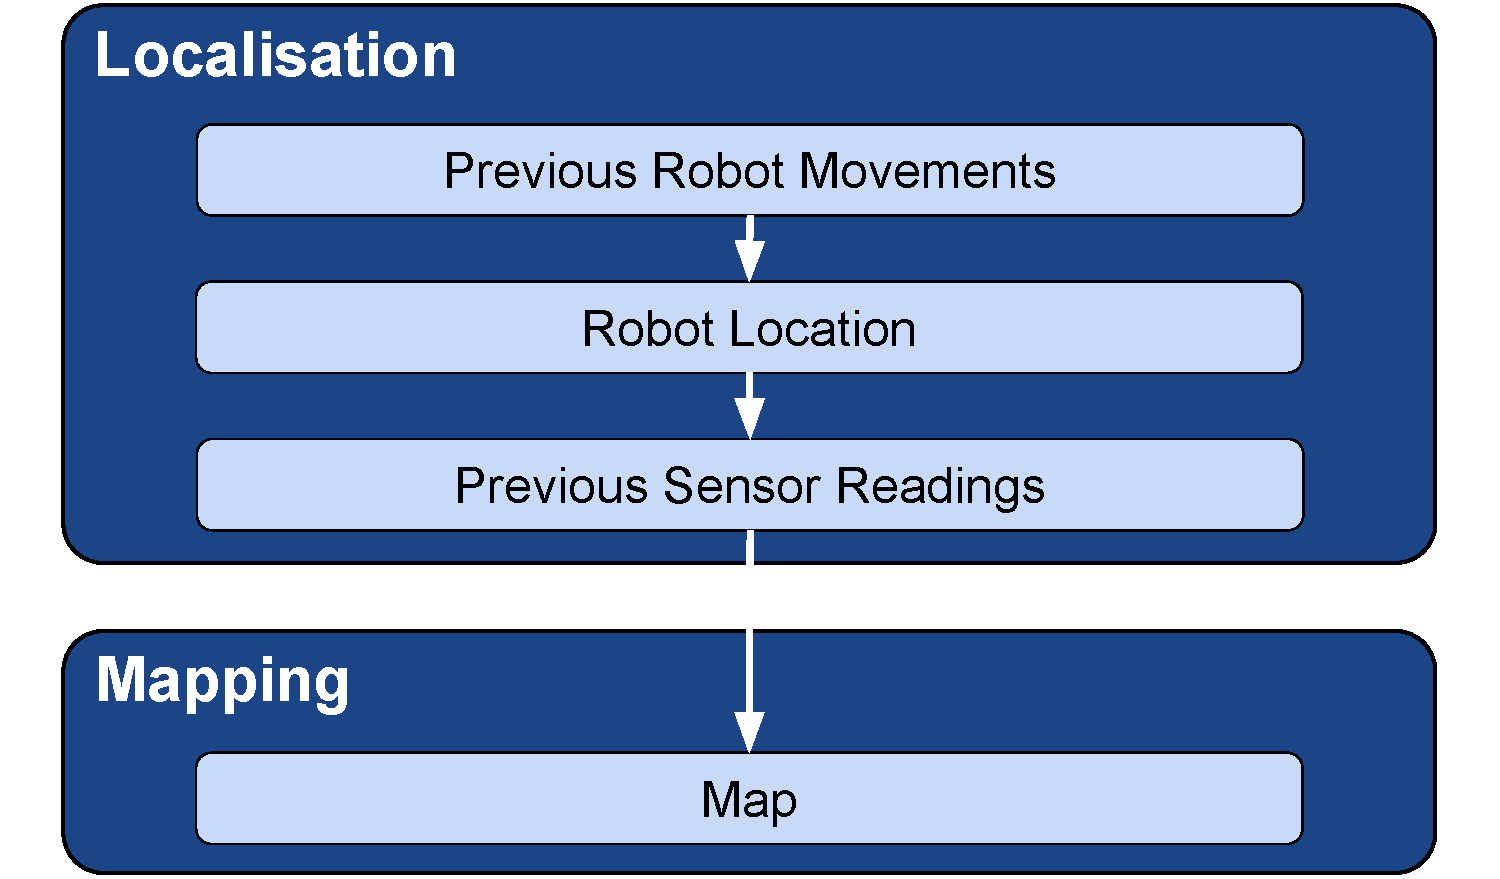
\includegraphics[width=0.8\textwidth]{figures/1Problem_analysis/Bayes_net.pdf}
    \caption{Illustration of Bayes net for a \gls{SLAM} scenario at a single point in time. In practice, the net continues for all previous and future points in time.}
    \label{fig:bayer_net}
\end{figure}

As mentioned, \gls{SLAM} can utilise different implementations such as the Extended Kalman Filter (\gls{EKF}) and the Particle Filter. The \gls{EKF} finds the smallest mean quadratic error of the system state based on features or landmarks in the environment, while assuming that any measurement errors are Gaussian random variables. The outcome of the mapping using the \gls{EKF} is usually a feature-based map, which can consist of points or lines indicating the outline of objects. The Particle Filter does not need feature detection or use of landmarks, but instead uses a set of particles to represent a probabilistic distribution of the system state, given noisy measurements. \cite{SLAM:ExtendedKalman_Particle}

The sensors for obtaining data can be split into two; the sensor for determining the relative position of the robot, and the sensor for determining the distance and direction to the objects. The former is usually achieved from odometry sensors with which the robot can dead-reckon its location. The latter is more diverse in the possible sensing technologies, with cameras, LiDAR, and sound being feasible solutions. The sound based-approach, also known as echolocation, is further explored in the following section. 

% Ideothetic and allothetic

\subsubsection{Echolocation}\label{subsec:Echolocation}
The basic knowledge of acoustics can be applied in real-life scenarios, such as music production, speech recognition, or, more contextually, echolocation. The latter is a scientific field of research on how sound that propagates through a medium and reflects off surfaces can be recorded to estimate the surrounding environment. To give a literal dissection of the term "echolocation", it stems from the words "echo" and "location". An echo is defined as a reflected sound that reaches a listeners ear, and a location refers to localising some object. This means that it tackles the problem of localising objects (creating a map) using reflected sound. The origin of echolocation emerged in nature, where it has evolved for millions of years, and is still actively a part of several animal groups to this day. \cite{Echolocation:Echolocation_behaviour}

\textbf{Origin in Animals}\\
While most animals use vision as the primary sense to create a conception of the environment, some animals are dependent on sound in cases where the eyes are incapable. This could both be in case of low visibility or long range perception. Animals that apply this technique both live above and below water, and common examples are bats and cetaceans, respectively. Interestingly, some humans have also adapted the capability of echolocation, especially inherently blind people. \cite{Echolocation:Echolocation_behaviour}

Turning the focus on the prime example in this field, i.e. bats, the way that echolocation is achieved consists of sending a pulse with a certain frequency, and capturing a reflected variation of that pulse, as seen in Figure \ref{fig:bat_echolocation}. The captured signal can then be interpreted as a location and size of an object in the vicinity of the bat. This location is estimated from the time delay between emitting a signal and receiving the reflected signal, and the difference in hearing between the two ears. By sending several pulses with varying frequencies, the bat can also gauge the size of the object. The reason is that larger objects reflect lower frequencies with higher amplitude, whereas smaller objects reflect higher frequencies with lower amplitudes. As such, the bat can perceive its surroundings by creating a "sound" map, and, consequently, catch prey while avoiding walls and other obstacles. \cite{Echolocation:Echolocation_bats}

\begin{figure}[H]
    \centering
    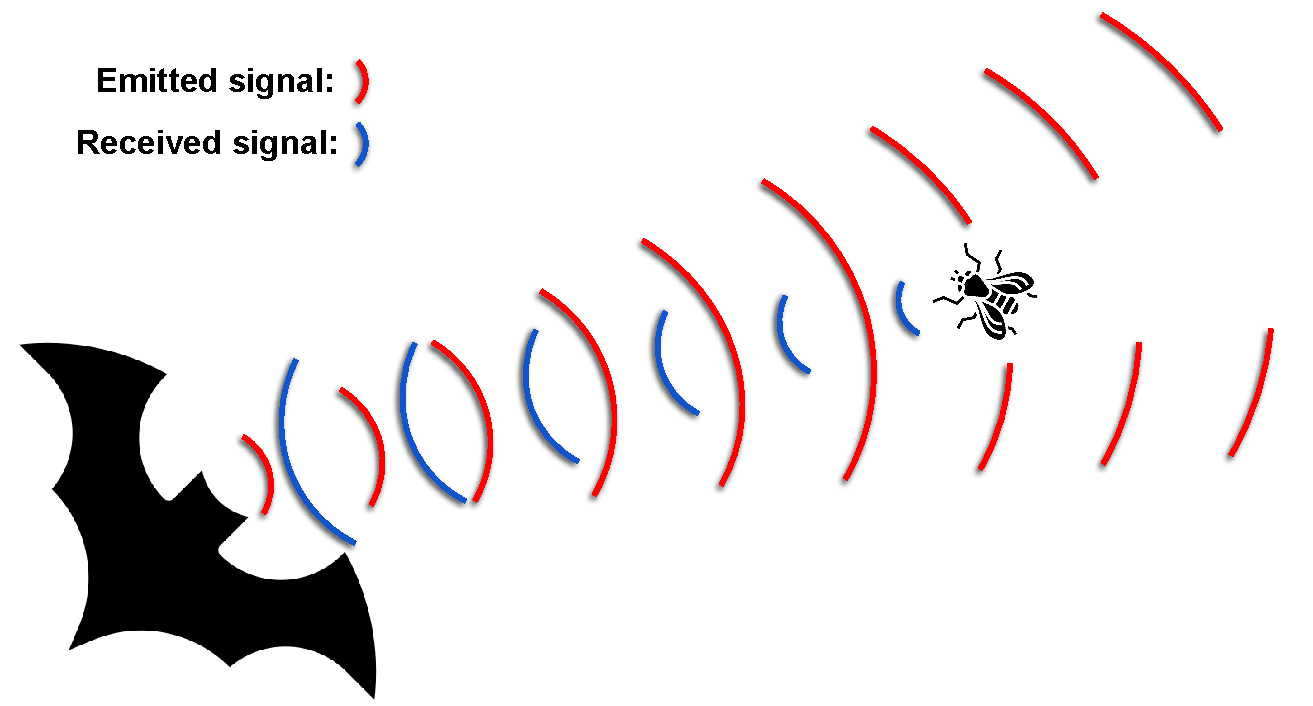
\includegraphics[width=0.8\textwidth]{figures/1Problem_analysis/Bat_echolocation.pdf}
    \caption{Illustration of a bat using echolocation to pinpoint where an insect is.}
    \label{fig:bat_echolocation}
\end{figure}

\textbf{Adaptation to Robotics}\\
In recent years, attempts to combine the fields of echolocation and robotics have been made in order to recreate the unique capability of bats and cetaceans. When taking the step from purely biological systems to robotic systems, there are several aspects to consider. Not only are there hardware components that need to be designed, constructed, and integrated into a combined setup, but there are also several software aspects that must be thoroughly considered and developed; especially because of the irregularity and unpredictability of the real world, caused by a dynamically changing environment. However, there have been very reasonable attempts of utilising the technology of echolocation in robotics to map the surroundings, as seen in e.g. \cite{Echolocation:Robat, Echolocation:Jesper_experiment}. In both of these, microphones are used to capture reflected signals emitted from a speaker on the robot. Signal processing methods are applied to determine the distance and direction of objects in the environment by isolating the desired signal from the noise. This attenuation of noise and accentuation of the desired signal covers a large proportion of the difficulties associated with acoustics in robotics. Therefore, an key requirement for such robotics solutions concern the Signal-to-Noise Ratio (\gls{SNR}) that the solution can obtain satisfying results for. How to deal with noise and the localisation of objects relative to the receiver will be introduced in Section REFERENCE. From the obtained data, a map must be generated based on techniques described in Section REFERENCE.


\subsection{Path Planning in Unknown Environment}
% Top level: Search pattern refers to the decision behind choosing a target point or direction.
% Middle level: Path planning refers to calculating the path of moving from A to B
% Bottom level: Motion planning refers to the computations behind robot locomotion and robot actuation


In autonomous navigation, one of the main challenges concerns determining how a robot is to move from one given location to another while manoeuvring the environment. The field that aims to solve this is path planning, which deals with the problem of computing a collision-free path to follow. 

The process of path planning can be distinguished as being either \textit{local} or \textit{global}, where one complements the other. Generally, a global path planner attempts to calculate an initial path between two points, based on the available information of the environment\footnote{This information can be given as a global map. \cite{PathPlanning:introduction_to_MR}}. Although literature tends to define this planner as only being applicable when the environment is entirely or partially known, it is in this project assumed that the planner can also perform in unknown environments, without guarantee of reaching destination if used by itself. This can e.g. be achieved by assuming a naive view of the world, where the environment is free of obstacles and without boundaries, resulting in the global path being the shortest euclidean distance to the goal. In the case of unforeseen changes during the path execution, such as obstacles obstructing the path, the local path planner can be applied to adapt to the global planner's initial path. These unexpected changes can be detected by the robot's local sensors. Due to these unique properties, the two path planners are often integrated together in order to ensure the best conditions for an obstacle-free path. Additionally, the desire to combine the path planners arises from the fact that the local path planner performs a more smooth path, while the global path planner has better capabilities with regards to escaping dead-ends\footnote{Dead-ends are often referred to as local minima.}. A typical architecture of a path planner, comprised of both the global- and local planner, can be seen in Figure \ref{fig:path_planner}. \cite{PathPlanning:introduction_to_MR}

% Mentioned that the global path planner is slightly different in case of unknown environment, and can be used even if the environment is unknown?
% Show example?

\begin{figure}[H]
    \centering
    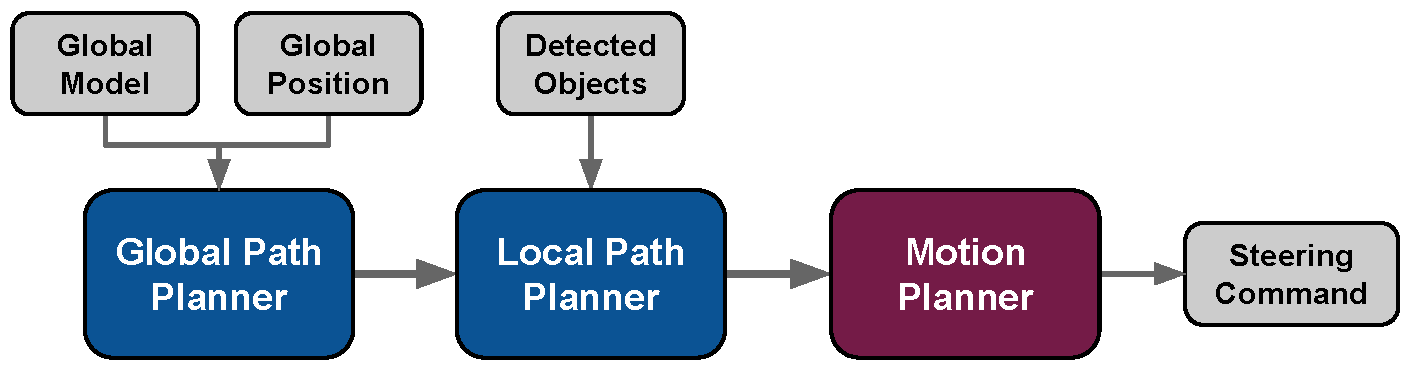
\includegraphics[width=0.8\textwidth]{figures/1Problem_analysis/General Path Planning.pdf}
    \caption{General architecture of a path planner illustrating how a global model, global position, and detected objects are transformed into steering commands by the two path planners. Adapted from \cite{PathPlanning:introduction_to_MR}.}
    \label{fig:path_planner}
\end{figure}

As can be seen, a steering command requires a global path to initially be generated from a global model, being the known information about the environment, and the robot's global position with respect to a fixed global frame. The path produced by this planner is then transferred to the local path planner, which adjusts the initial path according to the information of its local surroundings via its sensors, while following it as close as possible. After the adjusted path has been determined, signals must be sent to the robot's actuators to move along this path. However, these signals are not straightforward, and a method for how the robot physically moves is determined in the motion planner as seen on the right in Figure \ref{fig:path_planner}. Specifically, it calculates the motion, usually in the form of a velocity, over time, which creates a fast yet smooth response to the target location. To accomplish the desired response, a simple \gls{PID}-controller can be implemented, based on a few design criteria. This controller makes use of a closed-loop feedback system that compares the current location of the robot and the specified end location, such that it makes the robot decelerate to a halt exactly when reaching the point. 

The performance of a path planning method, as that shown in Figure \ref{fig:path_planner}, is influenced by the environment in which the robot is situated, which can be categorised as either known, partially-known, or unknown, and the expected status of objects, which can be either static or dynamic. As is the case in this project, the robot will not have any knowledge available about its environment prior to its deployment and operation, and the surrounding objects can change unexpectedly. Therefore, a navigation architecture that accounts for these characteristics has to be taken into account. 

\iffalse

Some of the most common path planning approaches, being \textit{Heuristic Search}, \textit{Dynamic Window Approach}, and \textit{Potential Fields}, will be explained in the following. 

\begin{itemize}
    \item \textbf{Heuristic Search:} This approach covers path planners that use heuristics\footnote{In this context, a heuristic is a function used to provide an estimated distance between a given location, referred to as a node, and the goal.} to guide the search for the most distance-optimal path to a goal. Using a heuristic, the search efficiency can be improved, since an estimation of the remaining path can be performed without having to explore it. One example of a prominent path planner is \textbf{A*}.   \cite{PathPlanning:Heuristic_Search}  

    \item \textbf{Dynamic Window Approach:} 
    
    \item \textbf{Potential Fields:} To explore the environment, path planners of these types make use of attractive and repulsive fields that guide the robot towards it goal. 
\end{itemize}

\fi

%Path planning is usually based on an approach that assumes a known environment, i.e. a well-defined map, which it can utilise to create the most optimal path for some application, e.g. directly from point A to point B or exhaustively through the entire room\footnote{This method is also known as coverage path planning.}. However, this is assuming that the map is already known, which is not always the case, especially not while performing \gls{SLAM}. As a matter of fact, path planning algorithms for this approach will not be optimal, as the spatial composition of the environment is neither known in advance nor a deterministic variable. In a mapping application, it is also evident that the path planning algorithm should traverse the environment without potentially missing any areas, such that a complete map can be constructed. 

\subsubsection{Exploration Schemes}
A multi-robot setup exploring a certain environment needs a method for tackling the efficiency problem. This means that the movements of the individual robots should be coordinated such that the most amount of terrain is covered in the least amount of time. As the number of robots increases, the problem becomes more complex as more variables are involved. To add to this, different areas could have different priorities, which would be indicated by some distribution. For simplicity, it can be assumed that each area is equally important, entailing a uniform distribution across the entire environment. 

There exists no ideal exploration scheme and the performance depends on the situation the robots are facing. Therefore, the choice of a scheme can be aided by considering three characteristics typically present in a multi-robot scenario. These are a central place, the size of the environment, and the presence of obstacles. The central place acts like a hub with which all robots can communicate to deliver information or obtain instructions. With respect to the size of the environment, one can deal with either a closed or open environment. In the latter case, the chance of a robot moving outside the range of the central place and thus losing connectivity must be accounted for. Lastly, obstructions present in the environment limit the robots' motion, and knowledge about their location could improve the exploration pattern. 

Generally, exploration schemes can be categorised by the following two extremes: \textit{Random Exploration} and \textit{Systematic Exploration}. The first scheme is ideal for closed environments in which the hub has connectivity to all robots. In this approach, the typical implementation is to have the robots wander the area until a goal or task has been achieved, which in this project is a map of the environment. Due to this search pattern being non-deterministic, its performance is determined statistically. The second of the two schemes relies on prior knowledge about the environment to systematically sweep it, and the robots may also memorise the areas they have visited in order to avoid exploring the same places multiple times, which is a typical implementation together with localisation and mapping. This scheme will solve a given task with certainty, unlike the prior case, and the duration of exploration is bounded when dealing with closed environments. Examples of these two extremes can be seen in Figure \ref{fig:exploration_schemes} using three agents.        

\begin{figure}[H]
    \centering
    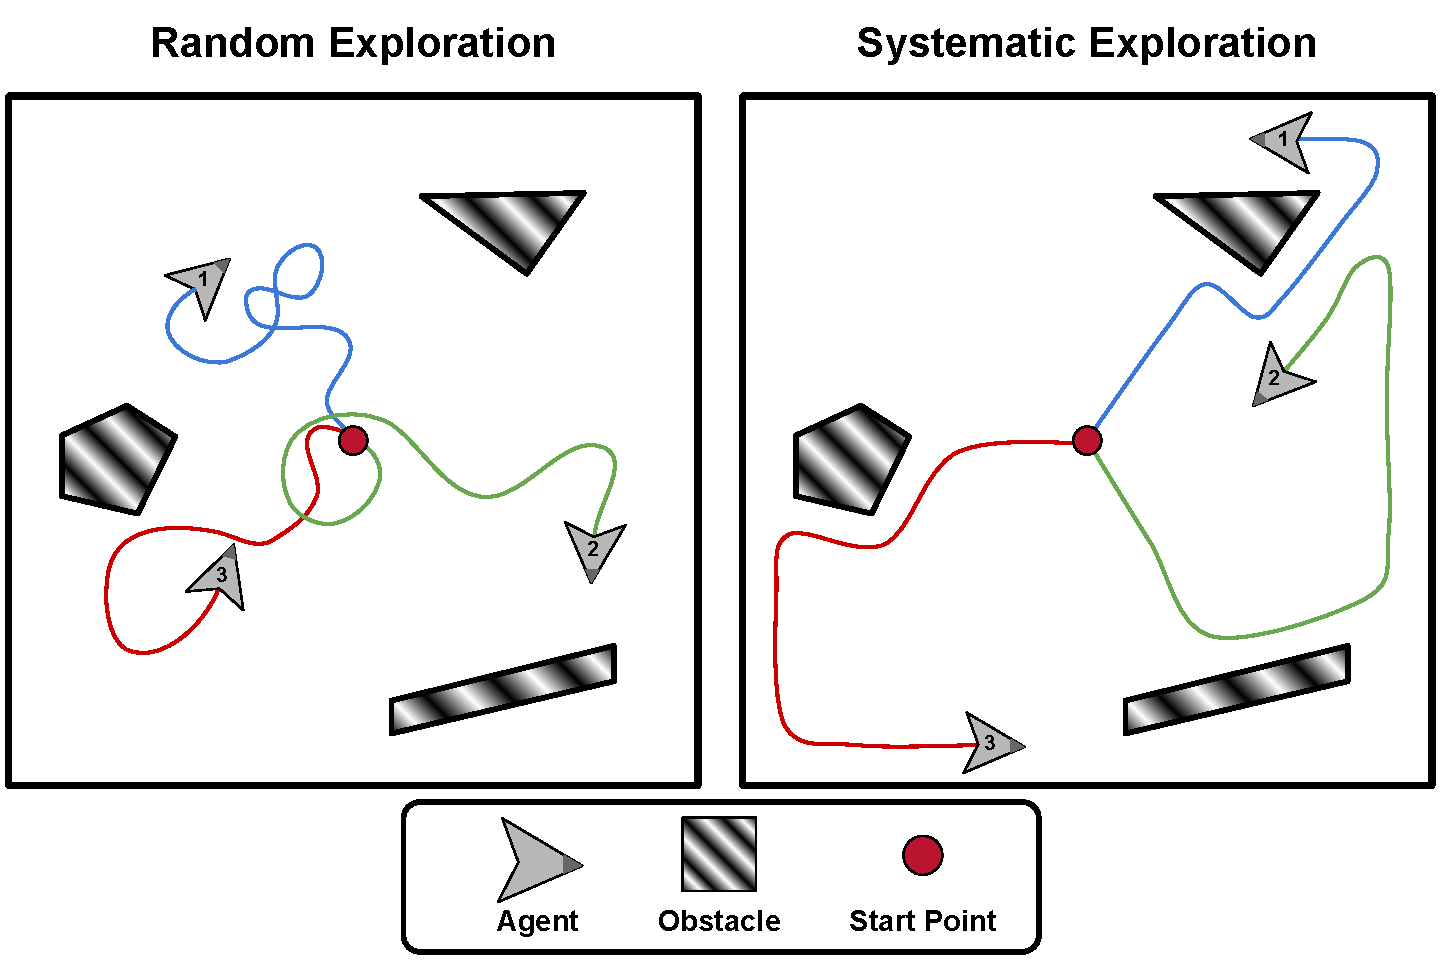
\includegraphics[width=0.9\textwidth]{figures/1Problem_analysis/Exploration Schemes.pdf}
    \caption{Example of multi-robot exploration in an environment with three objects. For random exploration, the robots explore the environment by moving in random directions and thus are shown to occasionally traverse a path that has already been explored. This is different from systematic exploration, as the robots here have prior knowledge of the environment and is thus shown to perform a more systematic exploration.} 
    \label{fig:exploration_schemes}
\end{figure}

It is important to note that there exists many different specialised exploration schemes between the two mentioned extremes, and their performance depends on the structure of the environment. \cite{PathPlanning:FundamentalSwarm}

% non-coordinated and coordinated

\subsection{Robotic Actuators}\label{subsec:RoboticActuators}
Previously, it was determined that sensors are required for a robot to perceive the environment. When the data from the sensors has been processed, the robot must enact the plan or series of actions it has prepared. To realise this, it is necessitated that a set of actuators is placed on the robot, so that the robot can actually interact with its environment. As with the robotic sensors, there are least needs to be two actuators for mapping via echolocation. As echolocation is an active way of sensing the environment, a loudspeaker is used to emit a sound before it can be measured by the sensor. Furthermore, it is evident that a mobile robot needs a mode of traversal, known as robot locomotion.


\subsubsection{Loudspeakers}\label{subsubsec:Loudspeakers}
%As previously mentioned, microphones are able to convert sound waves into electrical signals, however loudspeakers are capable of the opposite. Multiple types of speakers exist and this section explores some of the most prevalent ones. Moreover, the differentiation between audible and inaudible sound also affect the type of speaker.  

Similar to the microphone, a loudspeaker is also a transducer; however, it converts electrical energy to acoustical energy instead of the other way around. Loudspeakers emit signals, usually in the audible frequency range, which are perceived by humans as sound. This occurs from electrical energy bringing about movement in a diaphragm that produces acoustical energy. This diaphragm is often cone- or horn-shaped to direct the sound into a specific direction. A large problem of loudspeakers is caused by the fact that two acoustical outputs are emitted from it; one from the front and one from the back. As these outputs are out of phase, they will cancel if they are produced at the same time. Therefore, it is necessary to confine the backwards output by introducing a sealed enclosure and possibly phase shift or delay it. Moreover, sound behaves differently at low and high frequencies causing further complications. Even with the progress made through the years, an issue that remains is to acquire proper responses at the very low frequencies. Because of this, many loudspeakers only produce sound in a frequency range that is a subset of audible sound. Loudspeakers, like microphones, can as mentioned be directional, meaning the amplitude of the output changes based on the polar angle of it, which can be utilised for specific applications. This is only related to its physical size, and several loudspeakers could be combined to obtain a desired effect. Though, it should be noted that the directivity of loudspeakers is usually not constant across the entire pass-band. \cite{Acoustics:Handbook_of_Acoustics}

%%%%%%%%Ekstra om loudspeakers%%%%%%%%%%%%Kunne ikke finde så meget alligevel..
Multiple variations of speakers exist with one of the most common ones being the dynamic speaker. This works by having a voice coil connected to the diaphragm which generates vibrations when electrical current runs through it. This is due to the coil being encompassed by a magnet and therefore causing the coil to move when the magnetic field changes. This can be seen in Figure \ref{fig:Loudspeaker}. \cite{Acoustics:Audio_production}

\begin{figure}[H]
    \centering
    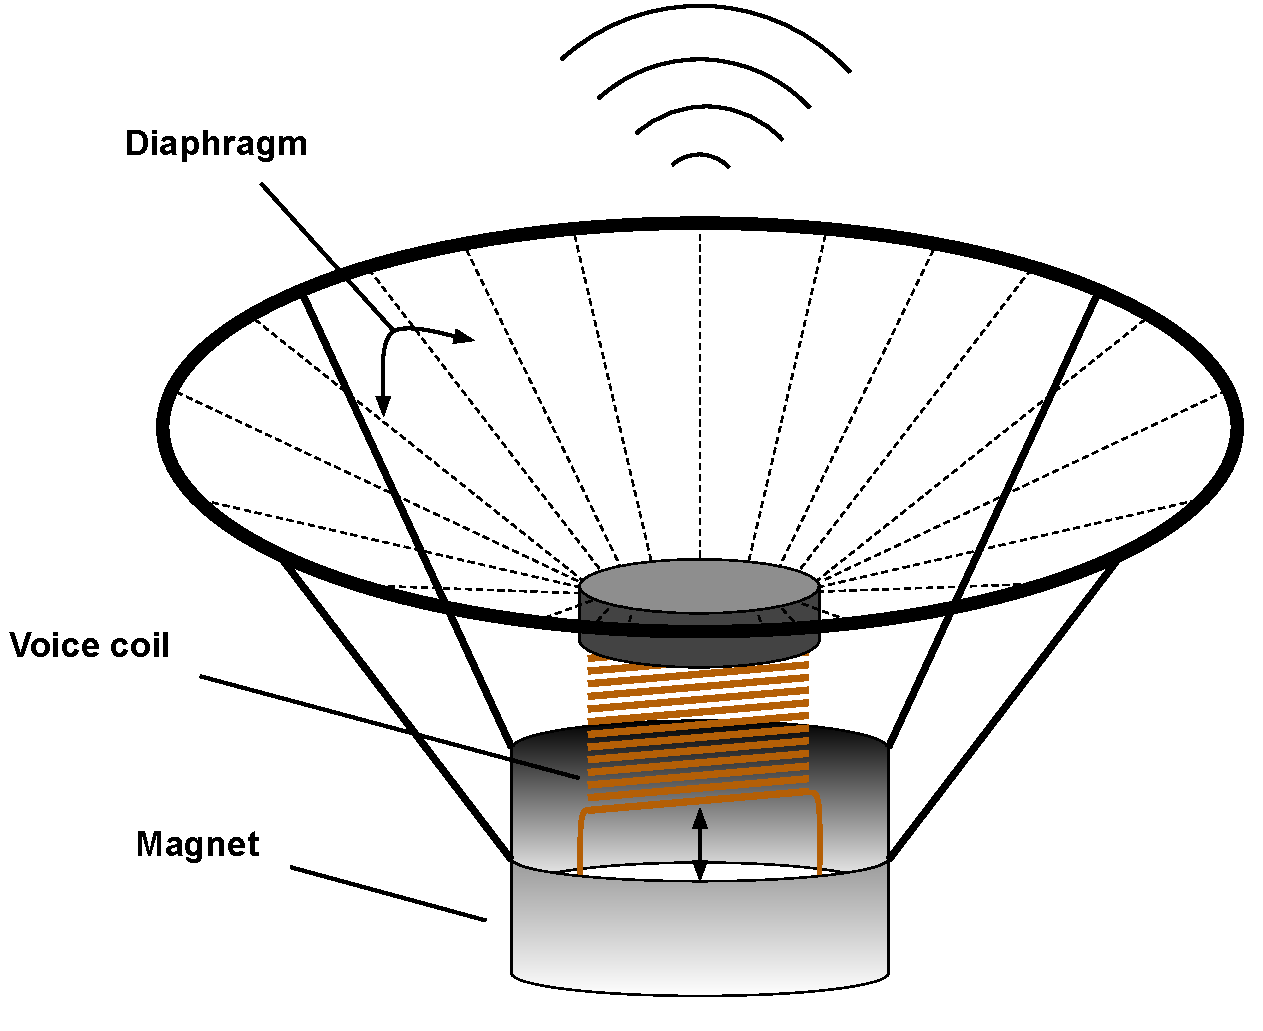
\includegraphics[width=0.6\textwidth]{figures/1Problem_analysis/loudspeaker.pdf}
    \caption{Simplistic view of a dynamic loudspeaker showcasing some of its internal components. Adapted from \cite{Acoustics:Audio_production}.}
    \label{fig:Loudspeaker}
\end{figure}



\subsubsection{Robot Locomotion}\label{subsubsec:RobootLocomotion}
In dealing with robot navigation, one area of interest is the robot locomotion. Or in other words, how the robot traverses a given environment context. In general and in correlation to search and rescue, three environment contexts can be set for the proposed solution. These are: 
(source: computational principles of mobile robotics)

\begin{multicols}{3}
    \begin{itemize}
        \Centering
        \item Terrestrial
        \item Aquatic
        \item Airborne
    \end{itemize}
\end{multicols}

As presented in \ref{sec:Search_and_Rescue} the context of this project is burning buildings. This context therefore only extends to indoor terrestrial or airborne traversal. 

Traversing in any of these contexts can be done utilising one or more of the following technologies, as solutions from Section \ref{subsec:ExistingSolutions} also presented:

\begin{multicols}{4}
    \begin{itemize}
        \Centering
        \item Wheels
        \item Tracks
        \item Legs
        \item Wings
    \end{itemize}
\end{multicols}

Manoeuvring in a burning building sets certain requirements for the mobility of the proposed solution. These are: It must be fast, It must be able to traverse over any object, It must be resilient to working environment.

Fast
Traversable in the environment
Resilient to the environment
Cost-effective
Scalable
Large operating time
Low inherent noise



These requirements limits the presented technologies, as not all of them are viable in this projects context. Specifically the tracked and legged technologies do not fit the requirements, as both of these are usually slow. (source: ) 

Wheeled robots are fast, require large a large circumference to manoeuvre over obstacles
Tracked robots are often slow, but can manoeuvre over almost any obstacles.
Legged robots are often slow and complex.
Non-fixed winged robots are very manoeuvre able in any environment, as they are not restricted by ground obstacles. 

